% ==========================================
% LatexRefinement Step Output: step4-03-31-25-tuesday-all-offset-final.tex
% Model: gemini-3.1-pro-preview
% Temperature: 0.35
% TopP: 0.93
% TopK: 35
% MaxOutputTokens: 65535
% ThinkingBudget: 32768
% ThinkingLevel: HIGH
% Prompt Tokens: 33'843
% Candidates Tokens: 23'877 (inkl. Thinking Tokens)
% Cached Tokens: 0
% Processed on: 2026-07-05 13:59:06
% ==========================================

% Primary Language: German
% End of the video: 01:33:02

\lecturechapter[7]{Dienstag}{31. Mär}{31. März 2026}{Grundstrukturen und das Auswahlaxiom}

\begin{nice-box}[Syllabus: Grundstrukturen und das Auswahlaxiom]
In dieser Vorlesung werden folgende Themen behandelt:
\begin{itemize}
    \item Das Banach-Tarski-Paradoxon als Motivation
    \item Formale Definition des Auswahlaxioms ($\text{AC}$) und seine Umformulierung
    \item Das Wohlordnungsprinzip ($\text{WOP}$) und Ordinalzahlen
    \item Der Beweis der Äquivalenz von Auswahlaxiom und Wohlordnungsprinzip über $\text{ZF}$
    \item Das Kuratowski-Zorn-Lemma ($\text{KZL}$) und seine Äquivalenz zu $\text{AC}$
\end{itemize}
\end{nice-box}

\section{Einführung und das Banach-Tarski-Paradoxon}

\begin{spoken-clean}[00:00:00 - 00:00:28]
Ja, jetzt. Guten Tag! Mein Name ist Fabian Ziltener. Ich vertrete Christian Urech heute für diese Vorlesung über Grundstrukturen und möchte mit einem Video anfangen. Dann sehen wir, was das mit Grundstrukturen zu tun hat. Also, hier ist es. Ich hoffe, dass Sie etwas hören. Vielleicht muss ich das Mikrofon dann hinhalten, aber mal schauen.
\end{spoken-clean}

\begin{meta-note}[Video: The Banach-Tarski Paradox]
Der Dozent spielt ein YouTube-Video von Vsauce mit dem Titel \qt{The Banach-Tarski Paradox} ab. Das Video ist auf Englisch.
\end{meta-note}

\begin{spoken-clean}[00:00:28 - 00:01:46]
{\itshape Hey, Vsauce. Michael here. There is a famous way to seemingly create chocolate out of nothing. Maybe you have seen it before. This chocolate bar is $4$ squares by $8$ squares, but if you cut it like this, and then like this, and finally like this, you can rearrange the pieces like so and wind up with the same $4$ by $8$ bar, but with a leftover piece, apparently created out of thin air.

There is a popular animation of this illusion as well. I call it an illusion because it is just that: fake. In reality, the final bar is a bit smaller. It contains this much less chocolate. Each square along the cut is shorter than it was in the original, but the cut makes it difficult to notice right away. The animation is extra misleading because it tries to cover up its deception. The lost height of each square is surreptitiously added in while the piece moves to make it hard to notice.

I mean, come on, obviously you cannot cut up a chocolate bar and rearrange the pieces into more than you started with. Or can you? One of the strangest...}
\end{spoken-clean}

\begin{meta-note}[Video pausiert]
Der Dozent pausiert das Video und wendet sich an die Studierenden.
\end{meta-note}

\begin{spoken-clean}[00:01:46 - 00:02:32]
Also, ich würde sagen, wir sind ja in der Schweiz, da stimmen wir über alles ab. Wir stimmen jetzt also mal ab: Wer ist dafür, dass man das kann? Eine Person, zwei, drei... ja, vielleicht zehn. Und wer ist dafür, dass man das nicht kann? Also Schokolade so aufspalten und dann wieder zusammenfügen, und am Schluss hat man mehr. Das ist eigentlich einigermaßen ausgeglichen.

Ich verrate Ihnen jetzt gleich die Antwort: Mit Hilfe des Auswahlaxioms kann man das. Es geht heute also um das Auswahlaxiom. Ich habe hier auch das Banach-Tarski-Paradox noch einmal hingemalt. Ich muss hier mal umschalten.
\end{spoken-clean}

\begin{meta-note}[Tafelübergang]

Der Dozent wechselt zur Tafel, auf der bereits eine Skizze zum Banach'-Tarski'-Paradoxon vorbereitet ist.

\end{meta-note}

\begin{math-stroke}[Das Banach-Tarski-Paradoxon]
\begin{center}
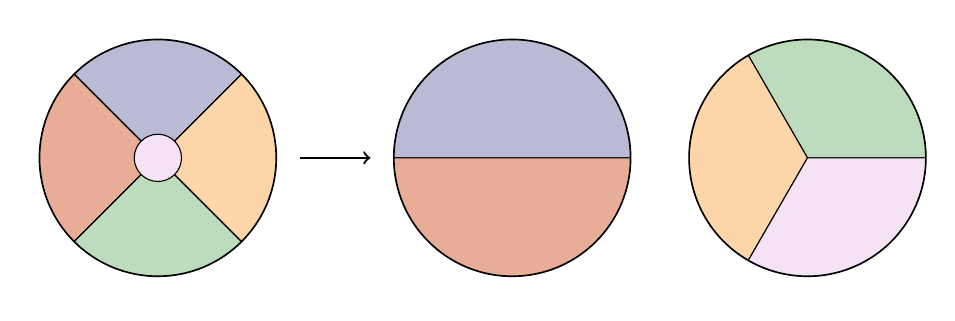
\begin{tikzpicture}[scale=1.5]
% \begin{ai-tikz-planner-invisible-content}
% 1. Background: Three circles representing the sphere before and after splitting.
% 2. Midground: Colored regions inside the circles to represent the pieces.
% 3. Foreground: Arrows indicating the transformation.
% \end{ai-tikz-planner-invisible-content}
    % First sphere (original)
    \draw[thick] (0,0) circle (1cm);
    \draw[fill=MidnightBlue!30] (0,0) -- (45:1) arc (45:135:1) -- cycle;
    \draw[fill=BrickRed!30] (0,0) -- (135:1) arc (135:225:1) -- cycle;
    \draw[fill=ForestGreen!30] (0,0) -- (225:1) arc (225:315:1) -- cycle;
    \draw[fill=BurntOrange!30] (0,0) -- (315:1) arc (315:405:1) -- cycle;
    \draw[fill=Plum!30] (0,0) circle (0.2cm); % Center piece

    % Arrow
    \draw[->, thick] (1.2, 0) -- (1.8, 0);

    % Second sphere (reconstructed 1)
    \begin{scope}[shift={(3,0)}]
        \draw[thick] (0,0) circle (1cm);
        \draw[fill=MidnightBlue!30] (0,0) -- (0:1) arc (0:180:1) -- cycle;
        \draw[fill=BrickRed!30] (0,0) -- (180:1) arc (180:360:1) -- cycle;
    \end{scope}

    % Third sphere (reconstructed 2)
    \begin{scope}[shift={(5.5,0)}]
        \draw[thick] (0,0) circle (1cm);
        \draw[fill=ForestGreen!30] (0,0) -- (0:1) arc (0:120:1) -- cycle;
        \draw[fill=BurntOrange!30] (0,0) -- (120:1) arc (120:240:1) -- cycle;
        \draw[fill=Plum!30] (0,0) -- (240:1) arc (240:360:1) -- cycle;
    \end{scope}
\end{tikzpicture}
\end{center}

Satz in Zermelo-Fraenkel + $\text{AC} = \text{Auswahlaxiom}$
\end{math-stroke}

\begin{spoken-clean}[00:02:32 - 00:03:40]
Das Banach-Tarski-Paradox sagt etwas Allgemeineres, aber eine Version davon besagt Folgendes: Sie können eine Kugel nehmen --- also einen dreidimensionalen Ball, in drei Dimensionen oder auch höher --- und die Kugel in fünf Teile aufspalten. Die habe ich hier so verschiedenfarbig gemacht. Und dann nehmen Sie zwei dieser Teile, also den blauen und den roten Teil, drehen diese, verschieben sie vielleicht noch und fügen sie wieder zusammen. Und Sie kriegen die gleiche Kugel wie da links: gleiche Größe, gleicher Radius.

Dann nehmen Sie die anderen drei Teile --- das sind dann orange, gelb und grün ---, drehen und verschieben diese, und kriegen dann wieder die gleiche Kugel wie links. Und das hier ist möglich! Das ist ein mathematischer Satz in Zermelo-Fraenkel plus AC. AC steht für Auswahlaxiom, Axiom of Choice.
\end{spoken-clean}

\subsection{Zermelo-Fraenkel-Axiome und das Auswahlaxiom}

\begin{spoken-clean}[00:03:40 - 00:04:46]
Ich habe von meinen Kollegen gehört, dass Sie die Zermelo-Fraenkel-Axiome schon behandelt haben. Weiß jemand noch eines? Kennt jemand noch ein Zermelo-Fraenkel-Axiom? Ja, bitte.
\end{spoken-clean}

\begin{student-interaction}[Studentenantwort]
Das Aussonderungsaxiom.
\end{student-interaction}

\begin{spoken-clean}[continued]
Das Aussonderungsaxiom, genau. Was sagt das?
\end{spoken-clean}

\begin{student-interaction}[Studentenantwort]
Wenn ich eine Menge $X$ habe und $\varphi$ ein $\mathcal{L}$-Satz ist, dann kann ich eine Menge aus den Elementen von $X$ machen, die die Bedingung $\varphi$ erfüllen.
\end{student-interaction}

\begin{spoken-clean}[continued]
Ja, genau. Man sondert halt all die Elemente aus, die eine bestimmte Bedingung erfüllen. Und das nullte --- was ist eigentlich das nullte Zermelo-Fraenkel-Axiom? Ja, bitte.
\end{spoken-clean}

\begin{student-interaction}[Studentenantwort]
Dass es eine leere Menge gibt.
\end{student-interaction}

\begin{spoken-clean}[continued]
Genau. Es gibt eine Menge, die keine Elemente enthält. Und dann gibt es halt noch ein paar andere. Und was alle brauchen, die sich nicht täglich mit Logik befassen, sondern mit anderer Mathematik, ist auch das Auswahlaxiom. Das ist quasi das letzte in der Liste. Je nach Zählung ist das dann das zehnte oder so. Und um dieses Auswahlaxiom geht es heute.
\end{spoken-clean}

\begin{spoken-clean}[00:04:46 - 00:06:20]
Ich sage Ihnen jetzt gleich in einem Satz, was das besagt. Das Auswahlaxiom sagt: Wenn Sie eine Menge von nichtleeren Mengen haben, dann können Sie gleichzeitig aus jeder dieser Mengen ein Element auswählen. Das klingt irgendwie sehr plausibel. Es scheint nicht sehr kontrovers zu sein. Aber aus dem Auswahlaxiom kriegen Sie dann eben zum Beispiel dieses Banach-Tarski-Paradox --- Sie können dann so eine Kugel aufspalten.

Warum heißt das jetzt Paradox? Respektive, das sollte ich die Leute fragen, die gesagt haben, es geht nicht mit dem Aufspalten. Wenn man das kann, kann man das mit der Schokolade übrigens auch. Theoretisch natürlich! Das hat nichts mit praktischem Schneiden zu tun --- praktisch geht das nicht. Ja, bitte.
\end{spoken-clean}

\begin{student-interaction}[Studentenantwort]
Das geht aber ja theoretisch nur aufgrund der unendlich vielen Anzahl der Punkte, die es gibt.
\end{student-interaction}

\begin{spoken-clean}[continued]
Ja, genau. Es geht nur theoretisch. Man muss irgendwie sehr, sehr genau schneiden. Es ist sehr ausgefranst. Diese Menge habe ich hier ein bisschen zackig gemalt --- Sie sollten sich das sehr ausgefranst denken. Man kann sie eben auch nicht explizit hinschreiben. Eine Sache bei diesem Auswahlaxiom ist, dass man die Auswahl, wie man die Elemente wählt, nicht explizit hinschreiben kann. Man braucht dafür eben das Axiom. Und hier ist es dann auch so: Man kann nicht hinschreiben, wie man die Menge aufspaltet, aber es gibt so eine Aufspaltung.

Aber warum heißt es Paradox? Anders gesagt: Die Leute, die gesagt haben, es geht nicht mit der Schokolade --- warum haben die das so gesehen? Warum denken Sie, es geht nicht? Irgendwie muss es ja einen Grund geben, dass das jetzt ein Paradox ist. Übrigens kommt das aus dem Griechischen: \qt{para} heißt gegen und \qt{doxa} heißt Anschein. Es ist gegen den Anschein. Es ist eben kein Widerspruch, es ist einfach nur gegen den Anschein. Warum? Ja, bitte.
\end{spoken-clean}

\begin{student-interaction}[Studentenantwort]
Also man würde erwarten, dass wenn man das zerschneidet und wieder zusammenschiebt, dass das Volumen gleich bleibt.
\end{student-interaction}

\begin{spoken-clean}[continued]
Genau. Wegen des Volumens ist es ein Paradox.
\end{spoken-clean}

\begin{math-stroke}[Der Grund für das Paradoxon]
\textbf{Grund:} $\leftarrow$ Volumen

\begin{explanation-of-steps}
Das Paradoxon widerspricht unserer Intuition über das Volumen. Wenn alle diese Teile ein wohldefiniertes Volumen hätten, dann ginge das nicht, da das Volumen additiv ist. Auf der rechten Seite hätten wir das doppelte Volumen. Der Trick ist, dass diese Teile gar kein Volumen haben. Sie sind nicht messbar im Sinne der Maßtheorie.
\end{explanation-of-steps}
\end{math-stroke}

\begin{spoken-clean}[00:06:52 - 00:07:30]
Der Grund, warum das viele Leute nicht so intuitiv finden, ist das Volumen. Wenn alle diese Teile ein wohldefiniertes Volumen hätten, dann ginge das eben nicht. Zumindest, wenn das Volumen auch noch gewisse Eigenschaften erfüllt, wie in der Maßtheorie --- nämlich endliche Additivität. Denn dann hätten Sie hier auf der rechten Seite das doppelte Volumen. Das Lustige ist aber: Diese Teile haben gar kein Volumen. Sie haben ein äußeres Maß, aber kein richtiges Maß. Daher ist das kein Widerspruch, sondern nur ein Paradox. Okay, gut. Das wollte ich zum Anfang sagen. Das ist eine Sache, die man aus dem Auswahlaxiom kriegt.
\end{spoken-clean}

\section{Das Auswahlaxiom und seine Äquivalenzen}

\subsection{Äquivalenzen zum Auswahlaxiom}

\begin{spoken-clean}[00:07:30 - 00:09:45]
Das ist jetzt etwas, was Sie vermutlich nicht verwenden werden, aber was Sie verwenden werden, ist eine andere Sache. Ich mache dann alles formal, aber zuerst schreibe ich mal ein bisschen auf, was die Relevanz dieses Auswahlaxioms in der Realität ist. Die Details folgen dann. 

Also, äquivalent über Zermelo-Fraenkel: Wenn man Zermelo-Fraenkel ($\text{ZF}$) annimmt, dann sind drei Sachen äquivalent. Nämlich das Auswahlaxiom ($\text{AC}$), dann das Wohlordnungsprinzip --- darüber werde ich heute mehr sagen. Dieses Wohlordnungsprinzip besagt, dass jede Menge wohlgeordnet werden kann. Was genau eine Wohlordnung ist, werde ich noch erklären. Etwas, was man dann hat, ist, dass je zwei Elemente verglichen werden können und jede nichtleere Teilmenge ein kleinstes Element hat. 

And dann gibt es noch das Dritte, was äquivalent über $\text{ZF}$ ist, nämlich das Kuratowski-Zorn-Lemma. Das sagt etwas über eine Halbordnung aus. (Wir werden Halbordnungen im Detail noch kennenlernen.) Es ist jetzt nicht so wichtig, was genau es besagt, aber aus diesem Kuratowski-Zorn-Lemma kriegen Sie dann eben zum Beispiel, dass jeder Vektorraum eine Basis hat. Und das ist dann etwas, was Sie in der Realität brauchen werden. \inlinemetanote{[Ein zentrales Resultat der Linearen Algebra, das ohne Auswahlaxiom nicht allgemein beweisbar wäre.]}
\end{spoken-clean}

\begin{math-stroke}[Äquivalenzen zum Auswahlaxiom]
\begin{itemize}
    \item $\text{AC}$ (Auswahlaxiom)
    \item $\text{WOP} =$ Wohlordnungsprinzip
    \item $\text{KZL} =$ Kuratowski-Zorn-Lemma $\implies$ Jeder Vektorraum besitzt eine Basis.
\end{itemize}
\end{math-stroke}

\begin{spoken-clean}[00:09:45 - 00:10:15]
Jeder Vektorraum besitzt also eine Basis. Vielleicht wird mein Kollege Urech noch etwas dazu sagen, wie man das beweist, oder es gibt vielleicht eine Übungsaufgabe dazu --- die gab es bei mir beim letzten Mal, als ich die Vorlesung gegeben habe. Wenn der Vektorraum endlichdimensional ist, dann können Sie die Basis konstruieren; das haben Sie vielleicht in der Linearen Algebra mit Hilfe von Induktion gemacht. Aber wenn der Vektorraum unendlichdimensional ist, dann wissen Sie a priori nicht, ob er eine Basis besitzt. Er besitzt sie eben nur wegen des Lemmas von Zorn --- oder Kuratowski-Zorn ---, was äquivalent zum Auswahlaxiom ist. Und das ist für mich ungefähr die Relevanz dieses Auswahlaxioms.
\end{spoken-clean}

\subsection{Das Auswahlaxiom}

\begin{spoken-clean}[00:10:15 - 00:12:30]
Okay, jetzt habe ich Ihnen hoffentlich ein bisschen einen Eindruck gegeben, was das ist und wozu es gut ist. Und jetzt mache ich es etwas genauer. Ich folge jetzt den Notizen, die ich damals geschrieben habe, und die sind im Internet. Vielleicht hat Herr Urech das angekündigt, und wenn nicht, können Sie diese in der Pause vielleicht mal suchen. Sie brauchen also jetzt nicht alles abzuschreiben, dazu gibt es ziemlich ausführliche Notizen. Hoffentlich stimmt die Nummerierung, das kann sich aber auch ändern.

Die Formulierung des Auswahlaxioms ist jetzt Punkt 1.1, auf den ich eingehen möchte. Ich werde es jetzt einfach gleich hinschreiben. Das Auswahlaxiom ist folgende Formel: Das hier bedeutet \qt{ist identisch gleich}. Ich weiß nicht, ob Herr Urech das auch so geschrieben hat. Es bedeutet Folgendes: Für alle $\mathcal{X}$ --- und ich mache jetzt so ein geschweiftes $\mathcal{X}$, weil ich mir das als ein Mengensystem denke. Das heißt, eine Menge von Mengen. Vielleicht haben Sie bei Herrn Urech gehört, dass alles eine Menge ist. Wenn Sie eine Menge haben und sich die Elemente davon anschauen, sind das auch wieder Mengen. Mathematisch gesehen ist das also nichts Spezielles, aber ich denke mir das als eine Menge von Mengen, und dafür mache ich so ein geschweiftes $\mathcal{X}$. Ich nenne das dann auch eine Kollektion von Mengen. 

Für jede Kollektion von Mengen, die nicht die leere Menge als Element enthält --- die leere Menge soll nicht darin liegen ---, gilt, dass es eine Funktion $f$ gibt. Diese Funktion heißt dann Auswahlfunktion. Sie muss eine Abbildung von dieser Kollektion zur Vereinigung all der Elemente der Kollektion sein.
\end{spoken-clean}

\begin{math-stroke}[Das Auswahlaxiom]
\begin{definition}[Auswahlaxiom]\label[definition]{def:auswahlaxiom}
Das \newterm{Auswahlaxiom} ($\text{AC}$) ist formal definiert als:
\begin{equation}
\text{AC} \equiv \forall \mathcal{X} \left( \emptyset \notin \mathcal{X} \rightarrow \exists f \left( f \in {}^{\displaystyle \mathcal{X}}\!\bigcup_{X \in \mathcal{X}} X \land \forall X \in \mathcal{X} \, (f(X) \in X) \right) \right)
\end{equation}
wobei $f$ eine \newterm{Auswahlfunktion} ist.
\end{definition}

\begin{explanation-of-steps}
\begin{itemize}
    \item $\mathcal{X}$ ist ein Mengensystem (eine Kollektion von Mengen).
    \item $\emptyset \notin \mathcal{X}$ stellt sicher, dass keine der Mengen in der Kollektion leer ist.
    \item $f$ ordnet jeder Menge $X \in \mathcal{X}$ ein Element aus genau dieser Menge $X$ zu ($f(X) \in X$).
    \item $\bigcup_{X \in \mathcal{X}} X$ ist die Vereinigung aller Elemente von $\mathcal{X}$.
\end{itemize}
\end{explanation-of-steps}
\end{math-stroke}

\begin{spoken-clean}[00:12:30 - 00:13:50]
Das hier ist meine Notation --- nicht nur meine, vielleicht hat Herr Urech sie auch eingeführt --- für die Vereinigung über alle Elemente. Man vereinigt alle Elemente hier drin. Die Elemente nenne ich jetzt einfach normal groß $X$. Ich vereinige also alle Mengen groß $X$, die in diesem geschweiften $\mathcal{X}$ liegen. Ich habe jetzt eine Abbildung von da nach da. Das ist die Notation für Abbildungen. Haben Sie das gesehen? Man schreibt das $X$ oft auch dahin, das ist die üblichere Notation, aber ich schreibe es jetzt mal so.

Oh, ja, das ist ein bisschen doof. Jetzt muss ich das noch irgendwie abstellen, das ist immer so eine Sache. Vielleicht einfach drücken, bis alles aus ist. Nein. Entschuldigung. Okay, hoffentlich kommt es nicht noch mal --- vielleicht doch.

Es gibt also so eine Auswahlfunktion, die von der ganzen Kollektion von Mengen zur Vereinigung geht, sodass für jedes $X$ in dieser Kollektion gilt, dass $f(X)$ in $X$ liegt. Und darum heißt es eben Auswahlaxiom oder Auswahlfunktion. So ein kleines $f$ nennt sich eine Auswahlfunktion. Es wählt aus jedem normalen $X$ --- ich mache das normale $X$ mal blau --- ein Element aus. Ich schreibe dafür mal klein $x$. Es wählt ein kleines $x$ aus dieser Menge aus. Okay?
\end{spoken-clean}

\begin{math-stroke}[Visualisierung der Auswahlfunktion]
\begin{center}
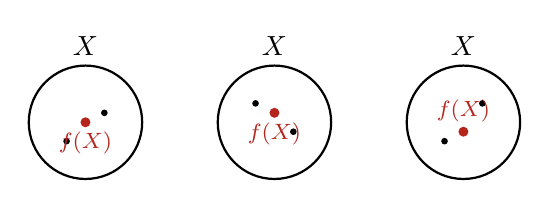
\begin{tikzpicture}[scale=1.2]
% \begin{ai-tikz-planner-invisible-content}
% 1. Background: Three circles representing sets X in \mathcal{X}.
% 2. Midground: Points inside the sets representing elements.
% 3. Foreground: A specific point in each set highlighted as the chosen element f(X).
% \end{ai-tikz-planner-invisible-content}
    % Set 1
    \draw[thick] (0,0) circle (0.6cm);
    \node[above] at (0, 0.6) {$X$};
    \fill (0.2, 0.1) circle (1pt);
    \fill (-0.2, -0.2) circle (1pt);
    \fill[BrickRed] (0, 0) circle (1.5pt) node[below, BrickRed] {\footnotesize $f(X)$};

    % Set 2
    \draw[thick] (2,0) circle (0.6cm);
    \node[above] at (2, 0.6) {$X$};
    \fill (1.8, 0.2) circle (1pt);
    \fill (2.2, -0.1) circle (1pt);
    \fill[BrickRed] (2, 0.1) circle (1.5pt) node[below, BrickRed] {\footnotesize $f(X)$};

    % Set 3
    \draw[thick] (4,0) circle (0.6cm);
    \node[above] at (4, 0.6) {$X$};
    \fill (3.8, -0.2) circle (1pt);
    \fill (4.2, 0.2) circle (1pt);
    \fill[BrickRed] (4, -0.1) circle (1.5pt) node[above, BrickRed] {\footnotesize $f(X)$};
\end{tikzpicture}
\end{center}
\end{math-stroke}

\subsection{Das allgemeine kartesische Produkt}

\begin{spoken-clean}[00:13:50 - 00:15:23]
Sie haben da also ein paar Mengen, vielleicht drei, und die haben einige Elemente. Jetzt nehme ich diese blaue Menge hier --- das ist vielleicht die erste --- und wähle halt etwas aus. Und das, was ich auswähle, ist eben $f(X)$. Das Rote hier ist $f(X)$, und $X$ ist die blaue Menge. Und das mache ich für alle gleichzeitig. Und dieses Axiom besagt, dass es eben so ein $f$ gibt. Gut.

Jetzt möchte ich dieses Auswahlaxiom mithilfe des kartesischen Produktes umformulieren. Ich nehme jetzt nicht an, dass Sie formal das kartesische Produkt einer beliebigen Kollektion von Mengen schon gesehen haben, das heißt, ich werde das jetzt erklären. Dieses kartesische Produkt verallgemeinert das von zwei Mengen, aber jetzt geht es eben gerade um unendlich viele Mengen. Dann wird es interessant! Wenn wir nur endlich viele nehmen, dann brauchen Sie kein Axiom; dann folgt aus der Induktion, dass es so ein $f$ gibt. 

Also, kartesisches Produkt. Man kann das so sehen: Wenn Sie eine Kollektion von nichtleeren Mengen haben und das kartesische Produkt davon nehmen, dann ist dieses auch wieder nicht leer. Die Elemente dieses kartesischen Produktes entsprechen genau solchen Auswahlfunktionen. Und das möchte ich jetzt erklären.

Zuerst einmal das Setting: Seien $I$ und so ein geschweiftes $\mathcal{X}$ Mengen. Das $I$ denken wir uns als eine Indexmenge. Wir indizieren dann Elemente aus gewissen Mengen mit Indizes darin. Und jetzt haben wir eine Abbildung $X$, die von groß $I$ nach dem geschweiften $\mathcal{X}$ geht. Die nimmt also ein $i$, und dann schreibe ich $X_i$ für einfach $X(i)$. Und das soll dann eine dieser Mengen sein. Man hat also eine Kollektion von Mengen. Aber formal gesehen ist das eine Abbildung, die einen Index nimmt und ihn in eine Menge abbildet.
\end{spoken-clean}

\begin{math-stroke}[Kartesisches Produkt einer Familie von Mengen]
Seien $I, \mathcal{X}$ Mengen, $X: I \to \mathcal{X}$ mit $X_i := X(i)$.

\begin{definition}[Kartesisches Produkt]\label[definition]{def:kartesisches-produkt}
Das \newterm{kartesische Produkt} der Familie $(X_i)_{i \in I}$ ist definiert als:
\begin{equation}
\bigtimes_{i \in I} X_i := \bigl\{ x \in {}^{\displaystyle I}\!\bigcup \mathcal{X} \;\big|\; \forall i \in I: x_i \in X_i \bigr\}
\end{equation}
wobei $x_i$ für $x(i)$ steht.
\end{definition}
\end{math-stroke}

\begin{spoken-clean}[00:15:23 - 00:17:30]
Und jetzt haben wir das Folgende: die Definition des kartesischen Produktes. Ich schreibe dafür so ein Kreuz. Letztes Jahr haben die Leute protestiert, dass es hier zu viele Kreuze gibt. Der Grund ist, schauen Sie, es geht alles irgendwie synchron: Sie haben ein kleines $x$, das liegt im großen $X$, und das große $X$ liegt im geschweiften $\mathcal{X}$. Mir gefällt das irgendwie. Aber wenn es Ihnen nicht gefällt, dann müssen Sie die Notation für sich persönlich ändern, das dürfen Sie gerne machen. Das Kreuz ist ein Kreuz, das möchte ich nicht ändern. Ich mache es jetzt dick. Das steht für das kartesische Produkt.

Ich schreibe jetzt einfach Kreuz $X_i$. Hier steht immer noch diese Abbildung $X$, schauen Sie, aber man darf das auch so schreiben, dann ist es ein bisschen intuitiver. Das hier ist effizient, und das hier rechts ist intuitiv: Produkt über alle Indizes, und dann schreibe ich hier dieses $X_i$. $X_i$ ist immer noch eine Menge. Jetzt scheint es ein bisschen intuitiver. Nehmen Sie zum Beispiel die Indexmenge $\{0, 1\}$, dann haben Sie ein $X_0 \times X_1$, okay?

Es ist das Folgende: Das sind alle Funktionen, die einen Index nehmen und ihn auf etwas in dieser Vereinigung hier abbilden. Und zwar so, dass für alle $i$ in der Indexmenge gilt: $x_i$ --- das ist wieder meine Lieblingsnotation für $x(i)$ --- liegt in groß $X_i$. Anders gesagt: Sie wählen für jeden Index ein Element aus dem entsprechenden großen $X_i$ aus.

Gut, ich könnte jetzt hier ein paar Beispiele machen, aber ich denke, Sie sollten sich das selbst anschauen; ich möchte hier nicht zu viel hinschreiben. Was ich noch sagen möchte, ist: Schauen Sie, wenn Sie jetzt nur zwei Mengen haben, $X_0$ und $X_1$, und Sie nehmen das kartesische Produkt --- was Sie vielleicht schon mal gesehen haben, denke ich, weil Sie ja die Zermelo-Fraenkel-Axiome hingeschrieben haben ---, woraus besteht das?
\end{spoken-clean}

\begin{student-interaction}[Studentenantwort]
Aus allen Paaren von Elementen von $X_0$ und $X_1$.
\end{student-interaction}

\begin{spoken-clean}[continued]
Ja, aus Paaren von Elementen, genau. Und ich habe so ein Zeichen verwendet wie Herr Halbeisen --- haben Sie das auch gemacht? Dieses eckige Zeichen für ein Paar. Okay, dann haben wir ein $\langle x_0, x_1 \rangle$. $x_0$ liegt in groß $X_0$, $x_1$ liegt in groß $X_1$. Und was ich jetzt sagen möchte, ist: Das, was ich jetzt hier neu gemacht habe, ist eben das Gleiche. Genauer gesagt können Sie dieses Paar mit der Funktion identifizieren, die $0$ auf $x_0$ und $1$ auf $x_1$ abbildet. Und diese Funktion liegt dann eben in diesem neuen kartesischen Produkt, wenn Sie gerade die Indexmenge $\{0, 1\}$ haben. Okay?

Das heißt, das Neue ist gleich dem Alten, wenn Sie nur zwei Mengen haben. Wenn Sie drei haben, können Sie sich auch so etwas überlegen. Aber das geht eben allgemeiner, auch wenn Sie unendlich viele Mengen haben. Wenn die Indexmenge $I$ unendlich ist, funktioniert das Neue eben auch, während das Alte scheitert. Und jetzt geht das nicht hoch... Es gibt nur die eine Tafel, vorher ging es gerade noch. Doch. Okay.
\end{spoken-clean}

\begin{math-stroke}[Spezialfall: Kartesisches Produkt zweier Mengen]
Für den Spezialfall $I = \{0, 1\}$ erhalten wir das gewohnte kartesische Produkt zweier Mengen:
\[
X_0 \times X_1 \ni \langle x_0, x_1 \rangle \leftrightarrow \begin{pmatrix} 0 \mapsto x_0 \\ 1 \mapsto x_1 \end{pmatrix} \in \bigtimes_{i \in I=\{0,1\}} X_i
\]
\end{math-stroke}

\begin{ai-note}[Mathematische Zuordnung]
Hier wird das geordnete Paar $\langle x_0, x_1 \rangle$ mit der Funktion $\begin{pmatrix} 0 \mapsto x_0 \\ 1 \mapsto x_1 \end{pmatrix}$ identifiziert ($\leftrightarrow$), anstatt eine Element-Beziehung ($\in$) zu verwenden, da die Funktion das Paar nicht als Element enthält, sondern das Paar repräsentiert.
\end{ai-note}

\subsection{Das kartesische Produkt einer Familie von Mengen}

\begin{spoken-clean}[00:17:30 - 00:19:30]
Und jetzt können wir das Auswahlaxiom eben auch damit formulieren. In meinen Notizen schreibe ich dann noch mehr dazu, warum diese zwei Sachen genau zusammenhängen. Das können Sie sich gerne durchlesen. Jetzt kommt also die Umformulierung des Auswahlaxioms mittels dieses Produkts. Ich schreibe dafür jetzt $\text{AC}'$. Das ist folgende Formel respektive folgender Satz: Für alle $I$ --- also Indexmengen ---, für alle geschweiften $\mathcal{X}$ und für alle großen $X$ --- das waren diese Abbildungen von der Indexmenge nach dem geschweiften $\mathcal{X}$ --- gilt Folgendes: Wenn für alle Indizes die Menge $X_i$ nicht leer ist, dann ist das kartesische Produkt der $X_i$ nicht leer.

Dieses neue Auswahlaxiom ist äquivalent zum alten über Zermelo-Fraenkel. Über Zermelo-Fraenkel gilt also: $\text{AC}$ ist äquivalent zu $\text{AC}'$. Das ist vielleicht das, was man in der Realität eher sagt. Man sagt einfach: Das kartesische Produkt von nichtleeren Mengen ist nicht leer. Das wird normalerweise so formuliert. Haben Sie dazu gerade Fragen?
\end{spoken-clean}

\begin{math-stroke}[Umformulierung des Auswahlaxioms]
\begin{definition}[Auswahlaxiom (Alternative Formulierung)]\label[definition]{def:auswahlaxiom-alt}
Das Auswahlaxiom lässt sich äquivalent formulieren als:
\begin{equation}
\text{AC}' \equiv \forall I \forall \mathcal{X} \forall X \in {}^{\displaystyle I}\!\mathcal{X} \left( (\forall i \in I \, (X(i) \neq \emptyset)) \rightarrow \bigtimes X \neq \emptyset \right)
\end{equation}
\end{definition}

\textbf{Über ZF:} $\text{AC} \leftrightarrow \text{AC}'$

\begin{explanation-of-steps}
Diese Formulierung besagt anschaulich: Das kartesische Produkt einer Familie von nichtleeren Mengen ist selbst nicht leer. Ein Element dieses kartesischen Produkts ist genau eine Auswahlfunktion, die aus jeder Menge $X_i$ ein Element auswählt.
\end{explanation-of-steps}
\end{math-stroke}

\begin{spoken-clean}[00:19:30 - 00:21:00]
Jetzt möchte ich ein bisschen erklären, wann man das Auswahlaxiom überhaupt braucht und wann nicht. Wie gesagt: Wenn Sie eine endliche Indexmenge haben, brauchen Sie es nicht. Dann können Sie mit Induktion zeigen, dass Sie aus endlich vielen Mengen endlich viele Elemente auswählen können. Und wenn Sie ein Merkmal haben, das ein Element aus jeder Menge eindeutig kennzeichnet oder charakterisiert, dann brauchen Sie das Auswahlaxiom ebenfalls nicht.

Hierzu eine Bemerkung als Beispiel: Wenn Sie eine Abbildung in die Potenzmenge von $\omega$ haben --- haben Sie dieses Zeichen $\mathcal{P}$ schon gesehen? Potenzmenge, die Menge aller Teilmengen von $\omega$. Und zwar so, dass jedes $X_i$ nicht leer ist. Dann brauchen wir kein Auswahlaxiom, um für jedes $i$ ein kleines $x_i$ in groß $X_i$ zu finden, also für eine Auswahlfunktion. Wir brauchen es nicht, um zu zeigen, dass das Produkt all dieser $X_i$ nicht leer ist. Der Grund: Wir wählen $x_i \in X_i$ einfach als das kleinste Element. Der Punkt ist, dass es hier ein ausgezeichnetes Element gibt, das ein bestimmtes Merkmal hat --- nämlich, dass es das kleinste Element ist, die kleinste natürliche Zahl. Dieses groß $X_i$ ist ja eine Teilmenge von $\omega$, der Menge der natürlichen Zahlen. Die haben Sie auch schon gesehen, oder? Haben Sie auch $\omega$ geschrieben? Das ist die Menge, die es gemäß einem Axiom von Zermelo und Fraenkel gibt. Sie spielt die Rolle der Zahlen $0, 1$ und so weiter. Wenn also $X_i$ immer eine nichtleere Teilmenge von $\omega$ ist, dann nehmen Sie einfach die kleinste Zahl darin. Da brauchen Sie kein Auswahlaxiom, um ein Element auszuwählen. Es gibt eben Situationen, in denen Sie es nicht brauchen.

Eine anschauliche Art, wie man das veranschaulichen kann, hat mit Schuhen und Socken zu tun. Wenn Sie eine unendliche Kollektion von Schuhen haben --- immer ein Paar von Schuhen ---, dann brauchen Sie kein Auswahlaxiom, um bei jedem Paar einen Schuh auszuwählen. Warum? Wie machen Sie das ohne Auswahlaxiom? Ja, bitte.
\end{spoken-clean}

\begin{student-interaction}[Studentenantwort]
Man nimmt immer den linken Schuh.
\end{student-interaction}

\begin{spoken-clean}[continued]
Genau, Sie nehmen immer den linken Schuh. Da brauchen Sie kein Auswahlaxiom. Das ist dann ein spezielles Merkmal, dass es eben der linke Schuh ist. Ein Schuh ist links, der andere ist rechts. Wenn Sie jetzt Socken haben, geht das eben nicht --- ich nehme jetzt an, die zwei Socken sehen immer exakt gleich aus. Wenn Sie unendlich viele Paare von Socken haben, können Sie nicht einfach jeweils den \qt{linken} Socken nehmen. Das heißt, dann brauchen Sie eben das Auswahlaxiom. Es gibt also einen Unterschied zwischen Schuhen und Socken. Bemerkung: Schuhe versus Socken. Das ist übrigens nicht von mir, das ist von... wer hat das noch gleich gesagt? Russell hat das gesagt, der mit dem Paradox. Haben Sie das gesehen, das Russellsche Paradox? Ja, genau der. 

Okay, gut. Haben Sie noch Fragen zum Auswahlaxiom? Wir haben jetzt zwei Versionen, die über Zermelo-Fraenkel äquivalent sind. Ich mache jetzt nicht vor, warum das so ist. Vielleicht war das bei mir vor einem Jahr eine Übungsaufgabe; es ist, denke ich, nicht so schwierig zu zeigen. Ja?
\end{spoken-clean}

\begin{student-interaction}[Studentenfrage]
Ich habe irgendwie die Übersicht über die ganzen $X$ verloren. Könnten Sie noch mal...
\end{student-interaction}

\begin{spoken-clean}[00:21:00 - 00:22:30]
Oh. Also schauen Sie: Das hier hat so Füßchen, das Füßchen-$X$ ist das große $X$. Dann gibt es das Geschweifte. Das hier ist eine Menge, die ein Element vom geschweiften $\mathcal{X}$ ist. Das geschweifte $\mathcal{X}$ ist so ein Mengensystem, eine Kollektion von Mengen. Ich muss ja sagen, worin dieses große $X$ Werte annimmt. Alles muss irgendwie eine Menge haben, in der es Werte annimmt. Das ist das geschweifte $\mathcal{X}$. Und das große $X$ nimmt einen Index und ordnet ihm eine Menge zu. Das sollten Sie sich merken. Und diese Menge darf nicht leer sein. Das Auswahlaxiom in der Strich-Version sagt nun, dass wir ein kleines $x_i$ darin wählen können --- und zwar uniform, also nicht einfach nur für ein festes $i$, sondern für alle $i$ gleichzeitig. Das ist der Punkt.

Jetzt möchte ich auf diese Äquivalenz zwischen Auswahlaxiom, Wohlordnungsprinzip und Kuratowski-Zorn-Lemma eingehen. Ich gehe jetzt aber nur auf die ersten zwei ein. Das Auswahlaxiom habe ich hingeschrieben, jetzt kommt das Wohlordnungsprinzip, das besagt, dass jede Menge wohlgeordnet werden kann. Ich erkläre Ihnen gleich, was eine Wohlordnung ist. Es gibt dabei zwei zentrale Punkte: Der eine ist, dass Sie je zwei Elemente bezüglich der Wohlordnung vergleichen können. Der andere Punkt ist, dass jede nichtleere Teilmenge ein kleinstes Element hat. Okay.

Jetzt kommt also Abschnitt 4.2: Wohlordnungsprinzip. Und dann geht es auch noch um Ordinalzahlen. Die werden wir brauchen, um zu zeigen, dass man das Wohlordnungsprinzip aus dem Auswahlaxiom folgern kann. Ordinalzahlen verallgemeinern die natürlichen Zahlen $0, 1$ und so weiter. Die Menge der natürlichen Zahlen ist selbst auch eine Ordinalzahl, und zwar die kleinste unendliche. Es gibt also Ordinalzahlen, die unendlich groß sind. Das ist der Hauptpunkt daran.
\end{spoken-clean}

\begin{math-stroke}[Wann braucht man AC nicht?]
\begin{remark}[Wann braucht man $\text{AC}$ nicht?]
Sei $X: I \to \mathcal{P}(\omega)$ mit $X_i \neq \emptyset$ für alle $i \in I$.
Wir brauchen \emph{kein} $\text{AC}$, um zu zeigen, dass $\bigtimes_{i \in I} X_i \neq \emptyset$.
Dies gilt, da wir für jedes $i \in I$ aufgrund der Wohlordnung von $\omega$ explizit das kleinste Element $x_i \in X_i$ wählen können.
\end{remark}
\end{math-stroke}

\begin{didactic-insight}[Schuhe versus Socken (Russell)]
Bertrand Russell veranschaulichte das Auswahlaxiom mit folgendem Vergleich:
Hat man unendlich viele Paar Schuhe, braucht man kein Auswahlaxiom, um aus jedem Paar einen Schuh zu wählen (man nimmt z.B. immer den linken Schuh). Hat man jedoch unendlich viele Paar identischer Socken, gibt es keine solche explizite Regel. Um aus jedem Paar einen Socken zu wählen, benötigt man das Auswahlaxiom.
\end{didactic-insight}

\section{Wohlordnungsprinzip und Ordinalzahlen}

\subsection{Wohlordnungen}

\begin{spoken-clean}[00:22:30 - 00:25:00]
Jetzt möchte ich erklären, was das Wohlordnungsprinzip besagt, und dafür brauche ich folgende Definition. Ich führe hier noch eine kleine Notation ein. Sei $<$ eine binäre Relation auf einer Menge $A$. Das heißt, das hier ist eine Teilmenge von $A \times A$. $A \times A$ ist immer noch das kartesische Produkt der Menge mit sich selber --- das alte mit diesen Paaren. Jetzt folgt die Definition, was es bedeutet, dass das hier eine Wohlordnung ist. Ich nenne die Relation jetzt nicht groß $R$, sondern einfach $<$; das darf man ja, oder?

Ich erkläre zuerst, was es bedeutet, dass es eine strikte lineare Ordnung ist, und dann, was eine Wohlordnung ist. Es gibt hier zunächst die Bedingung der Trichotomie. Trichotomie bedeutet: Für alle $x$ und $y$ in $A$ gilt entweder $x < y$ oder $x = y$ oder $x > y$. Und \qt{entweder} bedeutet hier wirklich ein ausschließliches Oder. 

Dann der zweite Teil, die lineare Ordnung: Die Relation heißt strikte oder strenge lineare Ordnung auf $A$ genau dann, wenn sie transitiv ist und die Trichotomie erfüllt. Übrigens kommt das aus dem Griechischen: \qt{tricha} heißt drei und \qt{temno} heißt schneiden. Man schneidet die Sache in drei Teile, und diese schließen sich gegenseitig aus. Darum heißt es so. Okay, transitiv --- was heißt das noch gleich? Dass die Relation transitiv ist? Ja, bitte.
\end{spoken-clean}

\begin{student-interaction}[Studentenantwort]
Wenn $x < y$ und $y < z$, dann ist $x < z$.
\end{student-interaction}

\begin{spoken-clean}[continued]
Ja, umgekehrt. Wenn $x < y$ und $y < z$, dann ist $x < z$. Genau. Transitiv bedeutet also: Für alle $x, y$ und $z$ gilt, wenn $x < y$ und $y < z$, dann folgt daraus $x < z$. Übrigens bedeuten meine Pfeile hier meistens Implikation. Es kann auch mal ein Funktionszeichen sein, aber meistens ist es eine Implikation. Genau, das haben wir jetzt also.

Jetzt gibt es die nächste Bedingung, die besagt, was es bedeutet, ein minimales Element einer Teilmenge zu sein. Ich nehme jetzt eine Teilmenge $S$. Ein $x$ darin heißt minimal bezüglich meiner Relation genau dann, wenn für alle $y$ in $S$ gilt, dass $y$ nicht kleiner als $x$ ist. Es muss nicht zwingend ein eindeutiges minimales Element geben. Wenn ich eine lineare Ordnung habe, ist das zwar der Fall, aber im Allgemeinen muss das nicht so sein. Okay.

Dann Nummer 4: Wohlordnung. Die Relation heißt Wohlordnung --- und darum geht es ja ---, wenn sie all das andere erfüllt. Das heißt, es muss eine lineare Ordnung sein, man kann also je zwei Elemente vergleichen, und es muss zusätzlich so sein, dass jede nichtleere Teilmenge ein minimales Element besitzt. Jede nichtleere Teilmenge von $A$ besitzt also ein minimales Element. Das bedeutet Wohlordnung. Und um solche Wohlordnungen geht es jetzt. Haben Sie dazu eine Frage?
\end{spoken-clean}

\begin{math-stroke}[Wohlordnung]
Sei $<$ eine binäre Relation auf einer Menge $A$, d.h. $< \subseteq A \times A$.

\begin{definition}[Eigenschaften von Relationen]\label[definition]{def:relation-properties}
\begin{enumerate}[label=\textbf{(\roman*)}]
    \item \textbf{Trichotomie:} $\forall x, y \in A \colon$ entweder $x < y$ oder $x = y$ oder $x > y$.
    \item \textbf{(Strikte) lineare Ordnung:} $<$ ist eine strikte lineare Ordnung auf $A \iff <$ ist transitiv \& Trichotomie.
    \item \textbf{Transitivität:} $\forall x, y, z \in A \colon x < y \land y < z \implies x < z$.
    \item \textbf{Minimales Element:} Sei $S \subseteq A$. Ein Element $x \in S$ heißt \newterm{$<$-minimal} $\iff \forall y \in S \colon y \not< x$.
    \item \textbf{Wohlordnung:} $<$ ist eine \newterm{Wohlordnung} $\iff <$ ist eine lineare Ordnung \& $\forall S \subseteq A, S \neq \emptyset$ besitzt $S$ ein $<$-minimales Element.
\end{enumerate}
\end{definition}

\begin{definition}[Wohlordnungsprinzip]\label[definition]{def:wohlordnungsprinzip}
Das \newterm{Wohlordnungsprinzip} ($\text{WOP}$) besagt: Auf jeder Menge $A$ gibt es eine Wohlordnung.
\end{definition}
\end{math-stroke}

\subsection{Das Wohlordnungsprinzip}

\begin{spoken-clean}[00:25:00 - 00:26:30]
In meinen Notizen stehen dann auch noch ein paar Bemerkungen, die jetzt nicht so wichtig sind. Das Wohlordnungsprinzip, $\text{WOP}$, hat den Status eines Axioms, okay? Nicht eines Theorems, sondern eines Axioms. Das Wohlordnungsprinzip besagt: Jede Menge kann wohlgeordnet werden. Auf jeder Menge $A$ gibt es also eine Wohlordnung. Ich möchte jetzt erklären, warum dieses Wohlordnungsprinzip äquivalent zum Auswahlaxiom ist. Das ist das Ziel dieser Vorlesung. Es gibt ein Theorem, das besagt, dass diese beiden über Zermelo-Fraenkel äquivalent sind. Wenn Sie also zusätzlich Zermelo-Fraenkel annehmen, kann man das eine aus dem anderen herleiten.
\end{spoken-clean}

\subsection{Äquivalenz von Auswahlaxiom und Wohlordnungsprinzip}

\begin{spoken-clean}[00:26:30 - 00:28:30]
Die eine Richtung ist ziemlich einfach zu beweisen. Es gibt jetzt ein Theorem --- ich schreibe das mit großen Buchstaben, weil es ein metamathematisches Theorem ist. Das hat Herr Urech vielleicht nicht so explizit gesagt. Was ist denn ein Theorem mit Kleinbuchstaben? Ein Satz, den man aus den Axiomen herleiten kann, oder? Und ein Satz war eine Formel ohne freie Variablen, wo alle Variablen durch einen All- oder Existenzquantor gebunden sind. Was ich hier mit Großbuchstaben meine, ist eben ein bisschen etwas anderes. Das Theorem besagt Folgendes: In Zermelo-Fraenkel sind das Auswahlaxiom und das Wohlordnungsprinzip äquivalent. Das, was jetzt hier steht, ist keine Formel im Sinne der Logik erster Stufe, weil hier noch dieses Zeichen vorkommt. Weiß jemand noch, was dieses Zeichen bedeutet? Ja, bitte.
\end{spoken-clean}

\begin{student-interaction}[Studentenantwort]
Dass man aus dem Zermelo-Fraenkel-Axiomen das beweisen kann.
\end{student-interaction}

\begin{spoken-clean}[continued]
Genau. Es gibt einen Beweis dieser Äquivalenz aus Zermelo-Fraenkel. Und diese Aussage hier ist eben ein metamathematisches Theorem: dass es einen Beweis gibt, okay? Gut. Haben Sie dazu gerade Fragen?

Jetzt zum Beweis der Implikation. Dass man in Zermelo-Fraenkel aus dem einen das andere kriegt, ist einfach. Ich mache jetzt übrigens keinen formalen Beweis wie ganz am Anfang, weil das viel zu schwierig wäre. Was ich jetzt eigentlich mache, ist: Ich verwende den gödelschen Vollständigkeitssatz und argumentiere dann so, wie man das eben normalerweise macht. Das haben Sie vielleicht bei Herrn Urech gehört. Der Zweck dieses Vollständigkeitssatzes war, dass man in Anführungszeichen \qt{normal} argumentieren kann. Wir nehmen also an, das Wohlordnungsprinzip gilt, und dann zeige ich, dass das Auswahlaxiom gilt. Das ist nicht schwierig.

Erinnern wir uns, was das Auswahlaxiom bedeutete: Da hat man mit einer Menge von Mengen angefangen, dem geschweiften $\mathcal{X}$, die die leere Menge nicht enthält. Und die Aussage war, dass es eine Auswahlfunktion gibt. Das möchte ich jetzt zeigen. Sei das hier also eine Menge von nichtleeren Mengen. Ich möchte nun meine Auswahlfunktion definieren. Dazu brauche ich den Trick, den ich vorhin an einem Beispiel erwähnt habe: Wenn alle Elemente aus dem geschweiften $\mathcal{X}$ ein spezielles Element $x$ haben, das ein spezielles Merkmal besitzt, dann bin ich fertig. Und das spezielle Merkmal wird sein, das kleinste Element zu sein. Dafür verwende ich jetzt eben meine Wohlordnung.

Es geht wie folgt: Wegen des Wohlordnungsprinzips gibt es eine Wohlordnung --- ich nenne sie wieder einfach $<$ --- auf der Vereinigung all dieser Mengen. Das ist die Vereinigung über alle normalen $X$ im geschweiften $\mathcal{X}$. Darauf gibt es eine Wohlordnung. Dann definiere ich meine Auswahlfunktion wie folgt: Sie soll eine Menge aus der Kollektion nehmen und mir ein Element daraus geben, sie geht also in diese Vereinigung. Und $f(X)$ ist definiert als das $<$-minimale Element von $X$. Das ist eindeutig, weil ich eine Wohlordnung habe, und wegen der Trichotomie, also wegen des \qt{Entweders}. Es kann nicht gleichzeitig sein, dass das eine kleiner ist als das andere und umgekehrt. Das geht eben nicht. Ich nehme also einfach das kleinste Element. Diese Menge ist ja nicht leer, darum gibt es überhaupt ein Element; sonst wäre es schiefgegangen. 

Haben Sie dazu gerade Fragen? Das ist meine Auswahlfunktion. Jetzt habe ich also das Auswahlaxiom aus dem Wohlordnungsprinzip hergeleitet. Das hier ist eine Auswahlfunktion, und daher gilt $\text{AC}$. Das steht übrigens für Axiom of Choice.
\end{spoken-clean}

\begin{math-stroke}[Äquivalenz von AC und WOP]
\begin{theorem}[Metamathematisches Theorem]\label[theorem]{thm:ac-wop-equiv}
Über Zermelo-Fraenkel ($\text{ZF}$) gilt:
\[
\text{ZF} \vdash \text{AC} \leftrightarrow \text{WOP}
\]
\end{theorem}

\begin{short-proof}[Beweis der Implikation $\text{WOP} \implies \text{AC}$]
Annahme: $\text{WOP}$ gilt.
Sei $\mathcal{X}$ eine Menge von nichtleeren Mengen ($\emptyset \notin \mathcal{X}$).
Wegen $\text{WOP}$ gibt es eine Wohlordnung $<$ auf der Vereinigungsmenge $\bigcup \mathcal{X} = \bigcup_{X \in \mathcal{X}} X$.
Wir definieren die Auswahlfunktion $f: \mathcal{X} \to \bigcup \mathcal{X}$ durch:
\[
f(X) := \text{das } <\text{-minimale Element von } X
\]
Da $X \neq \emptyset$ und $<$ eine Wohlordnung auf $\bigcup \mathcal{X}$ (und damit auch auf $X$) ist, existiert dieses minimale Element und ist wegen der Trichotomie eindeutig bestimmt. Somit ist $f$ eine wohldefinierte Auswahlfunktion, und $\text{AC}$ gilt.
\end{short-proof}
\end{math-stroke}

\subsection{Ordinalzahlen}

\begin{spoken-clean}[00:28:30 - 00:30:10]
Jetzt habe ich also diese Implikation bewiesen. Die andere Implikation ist schwieriger; dafür brauchen wir Ordinalzahlen. Das ist an sich etwas Interessantes. Haben Sie dazu Fragen? 

Die Ordinalzahlen verallgemeinern die natürlichen Zahlen. Die Idee ist, dass sie die Position in einer Rangliste angeben. In der Grammatik gibt es ja auch Ordinalzahlen --- so sollten Sie sich diese vorstellen. Es gibt dann den nullten, den ersten, den zweiten und den dritten. Wenn Sie zum Beispiel Sport machen, ist der nullte eben schneller als der erste, und der erste schneller als der zweite. Und so ist es mit den Ordinalzahlen auch: Sie sind linear geordnet. Was auch noch gut an den Ordinalzahlen ist: Wenn Sie irgendeine Menge von Ordinalzahlen haben, dann gibt es immer ein kleinstes Element. Es gibt immer den Schnellsten. Okay.

Aber es gibt eben dann auch noch den \qt{unendlichsten}. Und davon gibt es nicht nur einen! Nach dem nullten, dem ersten, dem zweiten und so weiter kommt dann der unendlichste. Und danach kommt der unendlich plus erste und der unendlich plus zweite. Irgendwann kommt dann der unendlich mal zweite, also unendlich plus unendlich, also $\omega + \omega$. Dann kommt $\omega \cdot 3$, und natürlich gibt es dann auch mal $\omega \cdot \omega$, und dann noch $\omega^\omega$ und $\omega^{\omega^\omega}$ und so weiter. Es hört nicht auf. Aber wir machen das nicht, wir brauchen das gar nicht. Ich wollte nur sagen: Es geht dann noch viel weiter.

Also, Ordinalzahlen. Definition: Sei $\alpha$ eine Menge. Ich sage zuerst einmal, was es bedeutet, dass die Menge transitiv ist. $\alpha$ heißt transitiv genau dann, wenn jedes Element davon auch eine Teilmenge ist. Für alle $\beta \in \alpha$ gilt also: $\beta$ ist eine Teilmenge von $\alpha$. Anders gesagt bedeutet das: Für alle $\gamma \in \beta$ gilt, dass $\gamma$ ein Element von $\alpha$ ist. Das hat natürlich ein bisschen was mit der Transitivität von vorhin zu tun. Sie können quasi die zwei Elementzeichen kontrahieren und erhalten wieder eins. 

Nummer 2: Wir nennen zwei Elemente $\beta$ und $\gamma$ vergleichbar genau dann, wenn $\beta \in \gamma$ liegt, oder $\beta = \gamma$ ist, oder $\gamma \in \beta$ liegt. Das ist ein inklusives Oder. Okay.

Und jetzt sage ich, was eine Ordinalzahl ist. $\alpha$ heißt Ordinalzahl genau dann, wenn es transitiv ist und je zwei Elemente vergleichbar sind. Für alle $\beta$ und $\gamma$ in $\alpha$ sind $\beta$ und $\gamma$ also vergleichbar bezüglich der Elementrelation. Und drittens: Jede nichtleere Teilmenge von $\alpha$ besitzt ein minimales Element.
\end{spoken-clean}

\begin{math-stroke}[Ordinalzahlen]
Sei $\alpha$ eine Menge.
\begin{enumerate}[label=\textbf{(\roman*)}]
    \item $\alpha$ heißt \newterm{transitiv} $\iff \forall \beta \in \alpha \, (\beta \subseteq \alpha)$.
    Äquivalent: $\forall \beta \in \alpha \, \forall \gamma \in \beta \, (\gamma \in \alpha)$.
    \item $\beta, \gamma \in \alpha$ heißen \newterm{vergleichbar} $\iff \beta \in \gamma \lor \beta = \gamma \lor \gamma \in \beta$.
\end{enumerate}

\begin{definition}[Ordinalzahl]\label[definition]{def:ordinalzahl}
$\alpha$ ist eine \newterm{Ordinalzahl} $\iff$
\begin{enumerate}[label=\textbf{(\alph*)}]
    \item $\alpha$ ist transitiv.
    \item $\forall \beta, \gamma \in \alpha$ sind $\beta, \gamma$ vergleichbar.
    \item Jede nichtleere Teilmenge von $\alpha$ besitzt ein minimales Element \inlinemetanote{[Anmerkung: bezüglich der Elementrelation $\in$]}.
\end{enumerate}
\end{definition}
\end{math-stroke}

\subsection{Die Klasse der Ordinalzahlen}

\begin{spoken-clean}[00:30:10 - 00:31:29]
Und dann definiere ich groß $\Omega$ als die Klasse aller Ordinalzahlen. Haben Sie bei Herrn Urech gehört, dass es einen Unterschied zwischen Klasse und Menge gibt? Nein? Also, ich mache hier geschweifte Klammern und lese das als Klasse. Formal gesehen gibt es das in Zermelo-Fraenkel nicht. In Zermelo-Fraenkel gibt es formal nur Mengen. Alles, was einen Variablennamen trägt --- ein $x$, ein $y$ oder dieses geschweifte $\mathcal{X}$ ---, wird als Menge interpretiert.

Wegen des Russellschen Paradoxons passiert es dann aber, dass es gewisse Dinge gibt, die keine Mengen sind, und diese nennen wir dann Klassen. Das ist jetzt der Fall bei diesem $\Omega$ hier. Was gab es denn für ein Ding, das keine Menge war? Ja, bitte.
\end{spoken-clean}

\begin{student-interaction}[Studentenantwort]
Die Menge aller Mengen.
\end{student-interaction}

\begin{spoken-clean}[continued]
Genau, die Menge aller Mengen gibt es eben nicht, und das nennt man dann die Klasse aller Mengen. Man muss mit diesen Zeichen ein bisschen aufpassen, wie man damit umgeht. Man darf damit nicht einfach alles machen. Aber man kann alles, was man damit macht, in wohldefinierte Formeln übersetzen. Okay? Ich mache jetzt Pause, nachher mache ich da weiter.
\end{spoken-clean}

\begin{math-stroke}[Die Klasse der Ordinalzahlen]
\begin{definition}[Klasse der Ordinalzahlen]\label[definition]{def:klasse-ordinalzahlen}
Wir definieren die Klasse aller Ordinalzahlen als:
\[
\Omega := \{ \alpha \mid \alpha \text{ ist Ordinalzahl} \}
\]
$\Omega$ ist eine \newterm{Klasse}, keine Menge.
\end{definition}
\end{math-stroke}

\begin{meta-note}[Pause]
Der Dozent kündigt eine Pause an. Nach der Pause wird die Vorlesung fortgesetzt.
\end{meta-note}

\begin{spoken-clean}[00:31:29 - 00:33:09]
Okay, wir machen weiter, bitte setzen Sie sich. Vor der Pause habe ich den Begriff einer Ordinalzahl definiert --- hier steht es noch einmal --- und gesagt, dass die Idee ist, dass diese Ordinalzahlen die Position in einer Liste angeben. Die natürlichen Zahlen sind Ordinalzahlen. Ich schreibe das mal als Bemerkung hin: Jede natürliche Zahl $n$ in $\omega$ --- $\omega$ ist immer noch die Menge der natürlichen Zahlen --- ist eine Ordinalzahl.

So eine natürliche Zahl besteht aus allen natürlichen Zahlen, die kleiner sind. $n$ ist also die Menge von $0$ bis $n-1$. Sprich: Die Zahl $0$ ist die leere Menge. So ist es definiert. Die $1$ ist die Menge, die genau die $0$ enthält. Die $2$ ist die Menge, die $0$ und $1$ enthält, und so weiter. Das sind alles Ordinalzahlen, das können Sie nachprüfen. Das ist nicht so schwierig.

Wenn Sie sich zum Beispiel die Menge $2$ anschauen und das Element $1$ nehmen: $1$ ist eben auch eine Teilmenge von $2$, weil $1$ genau die $0$ enthält, und die $0$ ist ja auch in $2$ enthalten. Die Idee ist eben, dass das eine Position in einer Liste angibt, und es hört nicht bei den endlichen Zahlen auf.
\end{spoken-clean}

\begin{math-stroke}[Natürliche Zahlen als Ordinalzahlen]
\begin{remark}[Natürliche Zahlen als Ordinalzahlen]
Für alle $n \in \omega$ ist $n$ eine Ordinalzahl. Es gilt:
\begin{align*}
n &= \{0, \dots, n-1\} \\
0 &= \emptyset \\
1 &= \{0\} \\
2 &= \{0, 1\} \\
&\vdots
\end{align*}
\end{remark}
\end{math-stroke}

\begin{spoken-clean}[00:33:09 - 00:34:45]
$\omega$ ist nämlich auch eine Ordinalzahl. Dass es transitiv ist, ist einfach zu sehen: Wenn Sie eine natürliche Zahl $n$ nehmen --- das ist mein $\beta$ in meinem $\alpha$, wobei $\alpha$ gleich $\omega$ ist ---, dann sind die Elemente von $n$ ja auch wieder natürliche Zahlen. Und es gibt eben immer ein kleinstes Element, das ist mehr oder weniger Induktion: Wenn Sie eine nichtleere Teilmenge der natürlichen Zahlen haben, gibt es ein kleinstes Element.

Es hört aber nicht bei unendlich auf, also bei $\omega$, sondern es geht noch viel weiter. Es gibt dann eben $\omega + 1$. Das ist der Nachfolger von $\omega$. Das haben Sie gebraucht, um die Menge der natürlichen Zahlen zu definieren --- dieses Symbol $S$ für \qt{successor}. Der Nachfolger ist die Menge $\omega$ vereinigt mit der Menge, die genau $\omega$ enthält. Wir tun also einfach $\omega$ noch als Element dazu. Das ist auch eine Ordinalzahl, das kann man sich überlegen. Insbesondere ist dieses Element hier eine Teilmenge davon, weil ja da wieder $\omega$ steht. Es ist also auch eine Teilmenge.
\end{spoken-clean}

\subsection{Unendliche Ordinalzahlen}

\begin{spoken-clean}[00:34:45 - 00:36:15]
Nach $\omega + 1$ kommt $\omega + 2$, sprich $\omega + 1 + 1$. Wir machen das Spielchen einfach nochmals: $S(S(\omega))$ und so weiter. Irgendwann kommt dann mal $\omega + \omega$. Bei mir war das eine Übungsaufgabe zu zeigen, dass das eine wohldefinierte Menge ist. Zuerst muss man definieren, was man meint. Man braucht das Ersetzungsaxiom, um zu zeigen, dass das sinnvoll ist oder um es überhaupt zu definieren. Das schreibt man dann als $\omega \cdot 2$.

Dann gibt es natürlich $\omega \cdot 3$ und so weiter. Und dann gibt es auch $\omega \cdot \omega$, also $\omega^2$, und nachher $\omega^3$. Und dann gibt es aber auch noch $\omega^\omega$ und $\omega^{\omega^\omega}$ --- mit Klammern so gesetzt, dass es interessant wird --- und so weiter. Wie das genau definiert ist, können Sie im Buch von Herrn Halbeisen und Gräf nachlesen. Das mache ich jetzt hier nicht vor, weil es nicht so wichtig ist. Wir brauchen die Ordinalzahlen hier nicht so explizit; wir brauchen sie jetzt nur als Hilfsmittel, um zu zeigen, dass aus dem Auswahlaxiom das Wohlordnungsprinzip folgt.
\end{spoken-clean}

\begin{ai-global-state-checkpoint-invisible-content}
% timestamp: 00:07:35
% topic: Ordinalzahlen und Unendlichkeit
% board_state: def:ordinalzahl-fortsetzung, def:klasse-ordinalzahlen
% next_goal: Eigenschaften der Klasse Omega und das Burali-Forti-Paradoxon
% open_loops: none
\end{ai-global-state-checkpoint-invisible-content}

\begin{math-stroke}[Unendliche Ordinalzahlen]
\begin{remark}[Unendliche Ordinalzahlen]
$\omega$ ist eine Ordinalzahl. Wir können weitere Ordinalzahlen durch die Nachfolgerfunktion $S$ konstruieren:
\begin{align*}
\omega + 1 &:= S(\omega) = \omega \cup \{\omega\} \\
\omega + 2 &= \omega + 1 + 1 = S(S(\omega)) \\
\omega + \omega &= \omega \cdot 2 \\
\omega \cdot 3, \dots, \omega \cdot \omega &= \omega^2, \omega^3, \dots, \omega^\omega, \omega^{\omega^\omega}, \dots
\end{align*}
\end{remark}
\end{math-stroke}

\begin{didactic-insight}[Besonderheiten transfiniter Ordinalzahl-Arithmetik]
Bei der Addition und Multiplikation transfiniter Ordinalzahlen muss man auf die Reihenfolge achten:
\begin{itemize}
    \item \textbf{Nicht-Kommutativität der Addition:} Es gilt $1 + \omega = \omega$, jedoch $\omega + 1 \neq \omega$ (da $\omega + 1$ das maximale Element $\omega$ besitzt, $\omega$ selbst aber kein maximales Element hat).
    \item \textbf{Rolle des Ersetzungsaxioms:} Um zu beweisen, dass Limes-Ordinalzahlen wie $\omega \cdot 2 = \bigcup_{n \in \omega} (\omega + n)$ existieren, benötigt man zwingend das Ersetzungsaxiom (\cref{ax:replacement}), da nur dieses garantiert, dass das Bild der Klassenfunktion $n \mapsto \omega + n$ über der Menge $\omega$ wieder eine Menge bildet.
\end{itemize}
\end{didactic-insight}

\subsection{Eigenschaften der Klasse der Ordinalzahlen}

\begin{spoken-clean}[00:36:15 - 00:37:50]
Um das zu erklären, brauche ich ein Theorem. Dieses Theorem besagt unter anderem, dass dieses groß $\Omega$ formal gesehen fast wie eine Ordinalzahl wirkt. In Zermelo-Fraenkel gilt nämlich Folgendes: Teil 1 besagt, dass für jedes $\alpha \in \Omega$ --- für jede Ordinalzahl --- gilt: $\alpha$ ist die leere Menge, oder die leere Menge ist ein Element von $\alpha$. Teil 2 besagt: Für alle $\alpha \in \beta$, wobei $\beta$ eine Ordinalzahl ist, gilt, dass $\alpha$ auch eine Ordinalzahl ist. Wenn ich also ein Element einer Ordinalzahl habe, ist es selbst auch eine Ordinalzahl. Teil 3 ist die Trichotomie: Für alle $\alpha$ und $\beta$ in $\Omega$ gilt entweder $\alpha \in \beta$, oder $\alpha = \beta$, oder $\beta \in \alpha$.

Dann gibt es noch Folgendes: Der Durchschnitt und die Vereinigung von Ordinalzahlen sind wieder Ordinalzahlen. Für alle Mengen $S$ von Ordinalzahlen gilt: Der Durchschnitt $\bigcap S$ ist eine Ordinalzahl. Und die Vereinigung $\bigcup S$ ist auch wieder eine Ordinalzahl. Bei diesem Durchschnitt muss man noch ein bisschen aufpassen: Wenn $S$ die leere Menge ist, dann war das bei mir formal als die leere Menge definiert. Philosophisch gesehen sollte der Durchschnitt von $S$, wenn $S$ leer ist, die Allmenge sein --- also die Klasse aller Mengen. In der Praxis kam es dann aber so heraus, dass es einfach die leere Menge war, weil man es anders irgendwie nicht definieren konnte. Es ist also kein Problem, wenn ich hier sage, der Durchschnitt ist ein Element von $\Omega$; es kommt nicht die Allklasse heraus.
\end{spoken-clean}

\begin{spoken-clean}[00:37:50 - 00:39:25]
Wohlgeordnetheit ist auch noch eine Eigenschaft: Für jede nichtleere Menge von Ordinalzahlen gibt es ein kleinstes Element. Es existiert ein minimales Element. Weil man jetzt eben die Eigenschaften 2, 3 und 5 hat --- die ich jetzt mal rot markiere ---, sieht das so aus, als ob dieses große $\Omega$ selbst eine Ordinalzahl wäre. Das erste ist Transitivität: Jedes Element von $\Omega$ ist ja auch eine Teilmenge, besagt Punkt 2. Punkt 3 besagt, dass je zwei Elemente vergleichbar sind --- hier gibt es sogar ein Entweder-Oder, vorher war nur ein Oder gefordert. Und Punkt 5 besagt Wohlgeordnetheit. Das waren genau die Bedingungen in der Definition einer Ordinalzahl.

Es kann aber nicht sein, dass $\Omega$ eine Menge ist, weil man sonst ein Problem bekommt. Bemerkung: $\Omega$ ist keine Menge. Das nennt sich das Burali-Forti-Paradoxon. Der Grund: Wäre es eine Menge, dann wäre es wegen der Punkte 2, 3 und 5 eine Ordinalzahl. Und wenn es eine Ordinalzahl ist, ist es ein Element von sich selber. Das geht aber nicht wegen der Trichotomie! Ordinalzahlen haben die Eigenschaft Entweder-Oder, sehen Sie hier. Das ist also ein Widerspruch zu diesem Entweder-Oder. Weil $\Omega = \Omega$ ist, kann es nicht auch ein Element von sich selber sein. $\Omega$ ist also keine Menge. Damit hat man das Problem, das Paradoxon, gelöst. Es ist halt größer als eine Menge. 

Haben Sie dazu Fragen? Das war übrigens nur eine Person: Cesare Burali-Forti war eine Person. Ich versuche jetzt, das hier abzustellen, hoffentlich funktioniert es dieses Mal. Entschuldigung, ich muss mal herausfinden, wie man das anders macht. Ah, ich hätte einfach... okay, gut, nächstes Mal.
\end{spoken-clean}

\begin{math-stroke}[Eigenschaften der Klasse der Ordinalzahlen]
\begin{theorem}[Eigenschaften von $\Omega$]\label[theorem]{thm:eigenschaften-omega}
In $\text{ZF}$ gilt:
\begin{enumerate}[label=\textbf{(\arabic*)}]
    \item $\forall \alpha \in \Omega \colon \alpha = \emptyset \lor \emptyset \in \alpha$
    \item $\forall \beta \in \Omega \, \forall \alpha \in \beta \colon \alpha \in \Omega$
    \item $\forall \alpha, \beta \in \Omega \colon \text{entweder } \alpha \in \beta \text{ oder } \alpha = \beta \text{ oder } \beta \in \alpha$
    \item $\forall S \text{ Menge von Ordinalzahlen} \colon \bigcap S \in \Omega, \bigcup S \in \Omega$
    \item $\forall S \subseteq \Omega, S \neq \emptyset \implies \exists \text{ minimales Element}$
\end{enumerate}
\end{theorem}

\begin{remark}[Burali-Forti-Paradoxon]
$\Omega$ ist keine Menge.
\textbf{Grund:} Wäre $\Omega$ eine Menge, so wäre $\Omega$ wegen \textbf{(2)}, \textbf{(3)} und \textbf{(5)} selbst eine Ordinalzahl, also $\Omega \in \Omega$. Dies ist ein Widerspruch zum \qt{entweder-oder} in \textbf{(3)}.
\end{remark}
\end{math-stroke}

\subsection{Hilfssatz und Pushforward einer Relation}

\begin{spoken-clean}[00:39:25 - 00:40:50]
Jetzt kommt ein Hilfssatz. Ich möchte immer noch zeigen, dass das Auswahlaxiom über Zermelo-Fraenkel das Wohlordnungsprinzip impliziert. Dazu brauche ich diesen Hilfssatz. In Zermelo-Fraenkel impliziert das Auswahlaxiom, dass es für jede Menge $A$ eine Ordinalzahl $\alpha$ und eine Bijektion von $\alpha$ nach $A$ gibt. Das ist der Hauptknackpunkt am ganzen Beweis. Wenn man das hat, geht es relativ schnell. Und das Schnelle mache ich jetzt vor. Okay?

Dazu muss ich jetzt etwas definieren: Ich definiere den Pushforward einer Relation unter einer injektiven Abbildung. Seien $X$ und $Y$ Mengen, $R$ eine binäre Relation auf $X$ und $u: X \to Y$ eine injektive Funktion. Dann definiere ich den Pushforward $u_* R$ als das Einzige, was ich tun kann: Ich möchte eine Relation auf $Y$ definieren. Was kann ich tun? Ich schaue mir die Paare $(u(x), u(x'))$ an, wobei das Paar $(x, x')$ in der Relation $R$ liegt. Das ist eine binäre Relation auf $Y$, also eine Teilmenge von $Y \times Y$, weil $u(x)$ und $u(x')$ in $Y$ liegen.
\end{spoken-clean}

\begin{spoken-clean}[00:40:50 - 00:42:10]
Dann Bemerkung 2: Wenn $R$ eine Wohlordnung auf $X$ ist und $u$ injektiv ist, dann ist dieser Pushforward $u_* R$ eine Wohlordnung auf dem Bild von $X$ unter $u$. Ich weiß nicht, wie Herr Urech das gemacht hat, aber ich schreibe hier eckige Klammern, weil ich das von der Funktionsanwendung an einem Punkt unterscheiden möchte. Ich schreibe in dieser Vorlesung eckige Klammern für das Bild. Das ist die Menge aller $u(x)$, wobei $x \in X$ liegt. Der Punkt ist, dass ich aus einer Wohlordnung wieder eine Wohlordnung auf der rechten Seite kriege. Und dann bin ich fertig! Das beweist, dass das Auswahlaxiom das Wohlordnungsprinzip impliziert. Die ganze Arbeit liegt also im Beweis des Hilfssatzes. Das möchte ich jetzt auch erklären. Haben Sie dazu eine Frage?
\end{spoken-clean}

\begin{math-stroke}[Hilfssatz und Pushforward einer Relation]
\begin{lemma}[Hilfssatz]\label[lemma]{lem:ac-implies-wop-hilfssatz}
In $\text{ZF}$ impliziert $\text{AC}$:
Für jede Menge $A$ existiert ein $\alpha \in \Omega$ und eine Bijektion $\alpha \to A$.
\end{lemma}

\begin{remark}[Pushforward einer Relation]
Seien $X, Y$ Mengen, $R$ eine binäre Relation auf $X$, und $u: X \to Y$ injektiv.
Wir definieren den \newterm{Pushforward} $u_* R$ als:
\[
u_* R := \{ (u(x), u(x')) \mid (x, x') \in R \}
\]
Dies ist eine binäre Relation auf $Y$.
\end{remark}

\begin{remark}[Erhaltung der Wohlordnung]
Wenn $R$ eine Wohlordnung auf $X$ ist und $u$ injektiv, dann ist $u_* R$ eine Wohlordnung auf dem Bild $u[X]$.
\end{remark}
\end{math-stroke}

\begin{student-interaction}[Studentenfrage]
Kleine Frage nur bei Beweis Hilfssatz steht da unten sei $A$ Menge, $A$ Element und dann $AC$?
\end{student-interaction}

\begin{proof}[Beweis des Hilfssatzes]
\begin{spoken-clean}[00:42:10 - 00:43:45]
Annahme. Ich nehme das Auswahlaxiom an, genau. Und am Schluss kriege ich dann die Bijektion zwischen $\alpha$ und $A$. Die nennt sich dann $v$. Gibt es andere Fragen?

Also, Beweis des Hilfssatzes. Bevor ich etwas Formales mache, möchte ich Ihnen die Idee des Beweises erklären. Was möchten wir? Für jede Menge gibt es ein $\alpha$ und eine Bijektion zwischen $\alpha$ und $A$. Die Idee ist: Wir zählen die Elemente aus $A$ auf. Wir wählen eines und nennen es das nullte. Dann nehmen wir ein nächstes und nennen es das erste. Und das nächste nennen wir das zweite, und so weiter. Wenn wir Glück haben, gibt es nur abzählbar viele Elemente, und wir haben sie vielleicht alle aufgezählt. Aber selbst wenn es überabzählbar viele Elemente hat --- vielleicht haben wir nach all diesen natürlichen Zahlen noch nicht alle aufgezählt. Dann machen wir einfach weiter mit $\omega$. Dann kommt das $\omega$-te. Und nachher das $(\omega+1)$-te, das $(\omega+2)$-te und so weiter. Irgendwann haben wir dann alle, und dann sind wir fertig. Das gibt uns die Bijektion: Null geht auf dieses nullte Element, eins geht auf das erste, zwei auf das zweite und so weiter. Das ist dann die Bijektion mit einer gewissen Ordinalzahl. So ist der Trick.
\end{spoken-clean}

\begin{spoken-clean}[00:43:45 - 00:45:14]
Jetzt mache ich das ein bisschen formal. Sei $A$ eine Menge. Annahme: Das Auswahlaxiom gilt. Ich betrachte jetzt nur den Fall, dass $A$ nicht die leere Menge ist; das ist der interessante Fall. Dann definiere ich $\mathcal{P}^*(A)$ als die Potenzmenge ohne die leere Menge. Wegen des Auswahlaxioms gibt es nun eine Auswahlfunktion für diese Potenzmenge. Sie wählt aus jeder nichtleeren Menge ein Element aus. Formal ging das in die Vereinigung, und diese Vereinigung ist einfach wieder $A$. Okay? Jetzt habe ich das Auswahlaxiom verwendet.
\end{spoken-clean}

\begin{ai-global-state-checkpoint-invisible-content}
% timestamp: 00:16:34
% topic: Beweis des Hilfssatzes (AC impliziert WOP)
% board_state: lem:ac-implies-wop-hilfssatz
% next_goal: Konstruktion der F-Mengen und Beweis der Bijektion
% open_loops: none
\end{ai-global-state-checkpoint-invisible-content}

\begin{math-stroke}[Beweis des Hilfssatzes: Setup]
Sei $A$ eine Menge. Annahme: $\text{AC}$ gilt.
Fall $A \neq \emptyset$.
Wir definieren:
\[
\mathcal{P}^*(A) := \mathcal{P}(A) \setminus \{\emptyset\}
\]
Nach $\text{AC}$ existiert eine Auswahlfunktion:
\[
f: \mathcal{P}^*(A) \to A
\]
\end{math-stroke}

\begin{spoken-clean}[00:45:14 - 00:46:55]
Dann definiere ich einen neuen Begriff, nämlich eine $F$-Menge. Ich weiß nicht, ob ich das Wort mag, aber so steht es im Buch von Herrn Halbeisen und Gräf. Ich würde es lieber eine $F$-Abbildung nennen, aber es heißt jetzt halt $F$-Menge. Denken Sie einfach an eine Abbildung. Eine $F$-Menge ist ein Paar $\langle \alpha, w \rangle$, wobei $\alpha$ eine Ordinalzahl ist und $w$ eine injektive Funktion von $\alpha$ nach $A$. Und zwar so, dass für alle $\gamma \in \alpha$ gilt: $w(\gamma)$ ist gegeben durch $f$ von dieser Menge hier. Hier kommt der Zusammenhang mit der Auswahlfunktion $f$ ins Spiel. Wir schauen uns das Bild von $\gamma$ unter $w$ an --- das mit den eckigen Klammern --- und nehmen das von $A$ weg. Dann wenden wir $f$ auf diese Differenzmenge an. Das gibt uns ein Element, das nicht in diesem Bild liegt. Das ist der Trick: Wir haben etwas Neues dazugenommen. Das wollen wir sowieso, weil die Funktion ja injektiv sein soll. Aber der Trick ist, dass wir genau dieses neue Element nehmen, das durch die Auswahlfunktion $f$ bestimmt wird. Jetzt habe ich also definiert, was eine $F$-Menge ist.
\end{spoken-clean}

\begin{math-stroke}[Definition der F-Menge]
\begin{definition}[F-Menge]\label[definition]{def:f-menge}
Eine \newterm{F-Menge} ist ein Paar $\langle \alpha, w \rangle$, wobei $\alpha \in \Omega$ und $w: \alpha \to A$ injektiv ist, sodass gilt:
\[
\forall \gamma \in \alpha \colon w(\gamma) = f(A \setminus w[\gamma])
\]
\end{definition}
\end{math-stroke}

\begin{spoken-clean}[00:46:55 - 00:48:30]
Jetzt kommt so eine Art Induktion. Man nimmt am Schluss die Vereinigung von allen $F$-Mengen, und das ist dann genau das, was wir wollen. Das entsprechende $\alpha$ ist unser $\alpha$ für die Bijektion. Dazu muss ich noch etwas definieren: Wenn ich zwei Mengen $X$ und $Y$ habe, dann schreibe ich $X \le Y$ genau dann, wenn $X \in Y$ oder $X = Y$ gilt.

Seien nun $\langle \alpha, v \rangle$ und $\langle \beta, w \rangle$ zwei $F$-Mengen. Dann gibt es eine Behauptung 1: Falls $\alpha \le \beta$ ist, dann ist die Einschränkung von $w$ auf $\alpha$ gleich $v$. Anders gesagt: $w$ ist eine Erweiterung von $v$. Es ist quasi die gleiche Funktion, einfach mit einem größeren Definitionsbereich. Hier habe ich $\alpha$ --- ich mache das $\alpha$ mal gelb --- und hier habe ich das größere $\beta$. Die Funktion wird einfach erweitert. Das hier ist $\beta$, das Rote. Hier habe ich das entsprechende $w$, und hier habe ich das $v$, das Gelbe. Beweisen werde ich das nicht, lesen Sie das selber nach. Es ist, glaube ich, auch nicht so kompliziert.
\end{spoken-clean}

\begin{spoken-clean}[00:48:30 - 00:49:40]
Dann Behauptung 2: Ich definiere jetzt $S$ als die Menge aller $F$-Mengen. Die Aussage ist genau, dass dies tatsächlich eine Menge ist. Wenn man es formal richtig sagt, bedeutet das: Es existiert eine Menge, deren Elemente genau die $F$-Mengen sind. Das beweise ich jetzt auch nicht. Sie können in meinen Notizen nachlesen, dass das wahr ist.
\end{spoken-clean}

\begin{math-stroke}[Eigenschaften von F-Mengen]
Wir definieren eine Relation:
\[
X \le Y \iff X \in Y \lor X = Y
\]

Seien $\langle \alpha, v \rangle$ und $\langle \beta, w \rangle$ F-Mengen.

\textbf{Behauptung 1:} Falls $\alpha \le \beta$, dann ist $w|_\alpha = v$.

\begin{center}
\begin{tikzpicture}[scale=1.5]
% \begin{ai-tikz-planner-invisible-content}
% 1. Background: Axes for Omega and A.
% 2. Midground: The function v on domain alpha in BurntOrange.
% 3. Foreground: The function w on domain beta in BrickRed, extending v.
% \end{ai-tikz-planner-invisible-content}
    % Axes
    \draw[->] (0,0) -- (3,0) node[right] {$\Omega$};
    \draw[->] (0,0) -- (0,2) node[above] {$A$};
    
    % Alpha and Beta on x-axis
    \draw (1, 0.1) -- (1, -0.1) node[below] {$\alpha$};
    \draw (2, 0.1) -- (2, -0.1) node[below] {$\beta$};
    
    % Function v (yellow/orange)
    \draw[thick, BurntOrange] (0,0) to[out=45, in=180] (1, 0.8);
    \node[BurntOrange, above left] at (0.5, 0.5) {$v$};
    
    % Function w (red)
    \draw[thick, BrickRed] (1, 0.8) to[out=0, in=200] (2, 1.5);
    \node[BrickRed, above left] at (1.5, 1.1) {$w$};
    
    % Dashed lines
    \draw[dashed] (1,0) -- (1, 0.8);
    \draw[dashed] (2,0) -- (2, 1.5);
\end{tikzpicture}
\end{center}

\textbf{Behauptung 2:} $S := \{ \langle \alpha, w \rangle \mid \langle \alpha, w \rangle \text{ ist F-Menge} \}$ ist eine Menge.
\end{math-stroke}

\begin{spoken-clean}[00:49:40 - 00:51:10]
Aus diesen zwei Behauptungen möchte ich jetzt den Hilfssatz beweisen --- also, dass es diese Bijektion gibt. Wie gesagt, der Trick ist, dass ich jetzt die Vereinigung von allen $F$-Mengen bilde. Ich definiere $\alpha$ als die Vereinigung aller $\beta$, wobei $\langle \beta, w \rangle$ eine $F$-Menge in $S$ ist. Das ist eine wohldefinierte Menge, weil $S$ eine Menge ist.

Und $v$ definiere ich als die Vereinigung aller $w$, für die $\langle \beta, w \rangle \in S$ gilt. Das ist die Vereinigung all dieser Graphen. Eine Funktion ist in dieser Vorlesung dasselbe wie ein Graph. In anderen Vorlesungen ist es ein Tripel, bestehend aus Definitionsbereich, Zielbereich und Graph, aber hier ist es einfach der Graph. Das hier ist dann die Vereinigung der Graphen --- also gelber Graph vereinigt mit rotem Graph und all den anderen. Jetzt habe ich hier also zwei Sachen hingeschrieben.
\end{spoken-clean}

\begin{math-stroke}[Konstruktion der Bijektion]
Wir definieren:
\begin{align*}
\alpha &:= \bigcup \{ \beta \mid \langle \beta, w \rangle \in S \} \\
v &:= \bigcup \{ w \mid \langle \beta, w \rangle \in S \}
\end{align*}
\end{math-stroke}

\begin{spoken-clean}[00:51:10 - 00:52:40]
Der Punkt ist nun Behauptung 3. Bei mir war das eine Übungsaufgabe, das zu beweisen. Ich mache es jetzt also nicht vor; es geht mir nur darum, dass Sie eine Idee haben, wie das überhaupt funktioniert. Es gibt hier drei Teile: Erstens ist $v$ eine Abbildung von $\alpha$ nach $A$. Es geht also nichts schief. Wenn Sie sich das Bild anschauen, ist das irgendwie klar: Weil $\beta$ eine Erweiterung von $\alpha$ ist, kriege ich den gleichen Wert. Wenn ich all diese Graphen vereinige, erhalte ich immer noch einen gültigen Graphen. An dieser Stelle verwende ich Behauptung 1.

Zweitens: $v$ ist injektiv. Das folgt aus der Injektivität der einzelnen Teile, weil eine $F$-Menge ja gerade so definiert war, dass das $w$ injektiv ist. 

Und drittens: $v$ ist surjektiv. Das ist das Interessante. Hier verwende ich, dass ich diese große Vereinigung gebildet habe --- dann habe ich eben alles abgedeckt.
\end{spoken-clean}

\begin{math-stroke}[Eigenschaften der konstruierten Abbildung]
\textbf{Behauptung 3:}
\begin{enumerate}[label=\textbf{(\roman*)}]
    \item $v$ ist eine Abbildung $\alpha \to A$.
    \item $v$ ist injektiv.
    \item $v$ ist surjektiv. \inlinemetanote{[Anmerkung: Wäre $v$ nicht surjektiv, so wäre $A \setminus v[\alpha] \neq \emptyset$, und die Auswahlfunktion lieferte ein Element $x := f(A \setminus v[\alpha])$. Man könnte $v$ dann auf $\alpha \cup \{\alpha\}$ erweitern, indem man $\alpha$ auf $x$ abbildet; nach \cref{def:f-menge} wäre $\langle \alpha \cup \{\alpha\}, v \cup \{\langle \alpha, x\rangle\}\rangle$ wieder eine F-Menge, also ein Element von $S$. Dann müsste aber $\alpha \cup \{\alpha\} \subseteq \alpha$ gelten, d.\,h.\ $\alpha \in \alpha$ --- ein Widerspruch (\cref{ax:foundation}).]}
\end{enumerate}
\end{math-stroke}

\begin{spoken-clean}[00:52:40 - 00:54:40]
Und das war's! Jetzt habe ich eine Bijektion zwischen $\alpha$ und $A$. Dass $\alpha$ eine Ordinalzahl ist --- habe ich das schon gesagt? Das hätte ich irgendwann noch sagen sollen, also sage ich es jetzt: $\alpha$ ist eine Ordinalzahl. Das folgt aus dem Theorem über $\Omega$. Wo steht es? Da, Teil 4: Die Vereinigung einer Menge von Ordinalzahlen ist eine Ordinalzahl. Und $\alpha$ ist ja genau die Vereinigung einer Menge von Ordinalzahlen, nämlich all dieser $\beta$.

Jetzt habe ich meine Bijektion zwischen einer Ordinalzahl und der beliebigen Menge $A$. Und das war der Hilfssatz! Der ist jetzt bewiesen --- modulo der Beweise der Behauptungen. Die finde ich jetzt nicht so interessant, die möchte ich Ihnen nicht zumuten. Haben Sie dazu Fragen? Es ging vielleicht alles ein bisschen schnell. Sie können gerne fragen, ja, bitte.
\end{spoken-clean}

\begin{math-stroke}[Abschluss des Beweises]
Da $\alpha$ die Vereinigung einer Menge von Ordinalzahlen ist, gilt nach \cref{thm:eigenschaften-omega} \textbf{(4)}:
\[
\alpha \in \Omega
\]
Somit haben wir eine Ordinalzahl $\alpha$ und eine Bijektion $v: \alpha \to A$ gefunden.
\end{math-stroke}
\end{proof}

\begin{ai-global-state-checkpoint-invisible-content}
% timestamp: 00:26:00
% topic: Abschluss des Beweises AC -> WOP
% board_state: thm:eigenschaften-omega, lem:ac-implies-wop-hilfssatz
% next_goal: Einführung des Kuratowski-Zorn-Lemmas
% open_loops: none
\end{ai-global-state-checkpoint-invisible-content}

\section{Das Kuratowski-Zorn-Lemma}

\begin{spoken-clean}[00:54:40 - 00:56:40]
Ich war dieses Mal ziemlich schnell. Das ist vielleicht nicht so ein gutes Zeichen, aber ich habe natürlich einige Sachen weggelassen. Ich glaube jedoch, das schadet nicht, weil das keine Beweise sind, bei denen Sie wirklich eine neue Idee sehen; Sie arbeiten einfach mit dem, was Sie haben. 

Was ich jetzt noch tun möchte, ist, das Kuratowski-Zorn-Lemma zu erklären. Ich habe ja versprochen, dass das Auswahlaxiom zu drei Sachen äquivalent ist: zu sich selber, zum Wohlordnungsprinzip und zum Lemma von Zorn. Das Kuratowski-Zorn-Lemma ist die Version des Auswahlaxioms, die Sie in der Realität tatsächlich sehen und anwenden werden. Darum schreibe ich das jetzt hin.

Da geht es um eine halbgeordnete Menge. Wir brauchen also den Begriff der Halbordnung. Ich mache das im schwachen Sinn, also mit $\le$, nicht mit $<$. Das beinhaltet Transitivität und Antisymmetrie: $x \le y$ und $y \le x$ impliziert $x = y$. Auf dieser halbgeordneten Menge hat man dann folgende Annahme: Immer wenn Sie eine Kette darin haben --- das ist eine linear geordnete Teilmenge ---, gibt es eine obere Schranke. Die Aussage des Zornschen Lemmas ist dann, dass die Menge ein maximales Element besitzt. Und dieses maximale Element ist dann zum Beispiel Ihre Basis des Vektorraums. So wenden Sie es an.
\end{spoken-clean}

\subsection{Halbordnungen und Ketten}

\begin{spoken-clean}[00:56:40 - 00:58:40]
Also, Kuratowski-Zorn-Lemma. Das hat wieder den Status eines Axioms; das Wort \qt{Lemma} sollte man sich also in Anführungszeichen denken. Ich brauche dafür den Begriff einer Halbordnung. Eine schwache oder nicht-strikte Halbordnung auf einer Menge $P$ --- $P$ steht für \qt{partial} --- ist eine binäre Relation $\le$ auf $P$ mit den folgenden Eigenschaften: Reflexivität hatte ich vorhin vergessen zu erwähnen, also $x \le x$ für jedes $x \in P$. Dann die Antisymmetrie, das ist das, was ich vorhin gesagt habe: Für alle $x, y \in P$ gilt, wenn $x \le y$ und $y \le x$, dann ist $x = y$. Und dann gibt es noch die Transitivität wie immer: Für alle $x, y, z \in P$ gilt, wenn $x \le y$ und $y \le z$, dann ist $x \le z$.

Wenn wir so etwas haben, nennen wir das Paar $(P, \le)$ eine halbgeordnete Menge. Eine schwache lineare Ordnung ist nun eine Halbordnung $\le$ auf $P$, sodass für alle $x$ und $y$ in $P$ gilt: $x \le y$ oder $y \le x$. Das ist fast wie vorher. Vorher war alles strikt, da hat man es ein bisschen anders formuliert, aber die Idee einer linearen Ordnung ist die gleiche: Man kann je zwei Elemente der Kette vergleichen.
\end{spoken-clean}

\begin{math-stroke}[Halbordnungen und Ketten]
\begin{definition}[Halbordnung]\label[definition]{def:halbordnung}
Eine \newterm{Halbordnung} auf einer Menge $P$ ist eine binäre Relation $\le$ auf $P$, sodass gilt:
\begin{enumerate}[label=\textbf{(\alph*)}]
    \item \textbf{Reflexivität:} $\forall x \in P \colon x \le x$
    \item \textbf{Antisymmetrie:} $\forall x, y \in P \colon x \le y \land y \le x \implies x = y$
    \item \textbf{Transitivität:} $\forall x, y, z \in P \colon x \le y \land y \le z \implies x \le z$
\end{enumerate}
\end{definition}

\begin{definition}[Schwache lineare Ordnung]\label[definition]{def:schwache-lineare-ordnung}
Eine \newterm{(schwache) lineare Ordnung} auf $P$ ist eine Halbordnung $\le$ auf $P$, sodass:
\[
\forall x, y \in P \colon x \le y \lor y \le x
\]
\end{definition}

\begin{definition}[Kette]\label[definition]{def:kette}
Eine \newterm{Kette} in $P$ ist eine Teilmenge $C \subseteq P$, sodass $\le$ eine lineare Ordnung auf $C$ ist.
\end{definition}
\end{math-stroke}

\subsection{Obere Schranken und maximale Elemente}

\begin{spoken-clean}[00:58:40 - 01:00:40]
Eine obere Schranke ist genau das, was sie sein soll: Eine obere Schranke für eine Teilmenge von $P$ ist ein Element $x \in P$, sodass für alle $y$ in dieser Teilmenge gilt: $y \le x$. Jedes Element ist kleiner oder gleich der oberen Schranke. Okay, das haben wir jetzt auch definiert.

Dann gibt es den Begriff eines maximales Elementes. Ein $x \in P$ heißt maximal genau dann, wenn für alle $y \in P$ gilt: Falls $y \ge x$, dann ist $y = x$. Es gibt also kein größeres Element. Das heißt aber nicht, dass dieses $x$ größer oder gleich jedem anderen Element ist! Das ist nicht so. Es gibt einfach nur kein Element, das strikt größer ist. Das ist ein wichtiger Punkt: Weil wir hier nur eine halbgeordnete Menge haben, spielt das eine Rolle. Bei einer Wohlordnung spielte das keine Rolle, aber hier eben schon. In meinen Notizen habe ich noch Bemerkungen dazu gemacht, die lese ich jetzt nicht vor.
\end{spoken-clean}

\begin{math-stroke}[Obere Schranke und maximales Element]
\begin{definition}[Obere Schranke]\label[definition]{def:obere-schranke}
Eine \newterm{obere Schranke} für $S \subseteq P$ ist ein $x \in P$, sodass:
\[
\forall y \in S \colon y \le x
\]
\end{definition}

\begin{definition}[Maximales Element]\label[definition]{def:maximales-element}
Ein Element $x \in P$ heißt \newterm{maximal} $\iff$
\[
\forall y \in P \colon y \ge x \implies y = x
\]
\end{definition}
\end{math-stroke}

\subsection{Formulierung des Kuratowski-Zorn-Lemmas}

\begin{spoken-clean}[01:00:40 - 01:02:40]
Und jetzt kommt das Kuratowski-Zorn-Lemma. Das kann ich jetzt formulieren: Sei $(P, \le)$ eine halbgeordnete Menge, und zwar so, dass für jede Kette $C$ in $P$ eine obere Schranke existiert. Dann besitzt $P$ ein maximales Element.
\end{spoken-clean}

\begin{math-stroke}[Das Kuratowski-Zorn-Lemma]
\begin{theorem}[Kuratowski-Zorn-Lemma ($\text{KZL}$)]\label[theorem]{thm:kzl-formal}
Sei $(P, \le)$ eine Halbordnung, sodass für jede Kette $C \subseteq P$ eine obere Schranke existiert. Dann besitzt $P$ ein maximales Element.
\end{theorem}
\end{math-stroke}

\subsection{Äquivalenz der Axiome}

\begin{spoken-clean}[01:02:40 - 01:04:40]
Es gilt nun folgendes Theorem: In $\text{ZF}$ sind äquivalent: erstens das Auswahlaxiom, zweitens das Wohlordnungsprinzip und drittens das Kuratowski-Zorn-Lemma. Dass die ersten beiden äquivalent sind, habe ich gerade bewiesen. Es ginge jetzt noch darum zu zeigen, dass das Auswahlaxiom und das Lemma von Zorn äquivalent sind. Damit werde ich jetzt aber wahrscheinlich nicht mehr anfangen, weil ich mir die Notizen dafür nicht ausgedruckt habe. Ich dachte nicht, dass ich so schnell bin.
\end{spoken-clean}

\begin{math-stroke}[Äquivalenz der Axiome]
\begin{theorem}[Äquivalenz in ZF]\label[theorem]{thm:aequivalenz-zf}
In $\text{ZF}$ sind äquivalent:
\begin{enumerate}[label=\textbf{(\alph*)}]
    \item $\text{AC}$ (Auswahlaxiom)
    \item $\text{WOP}$ (Wohlordnungsprinzip)
    \item $\text{KZL}$ (Kuratowski-Zorn-Lemma)
\end{enumerate}
\end{theorem}
\end{math-stroke}

\begin{ai-global-state-checkpoint-invisible-content}
% timestamp: 00:36:00
% topic: Kuratowski-Zorn-Lemma und Äquivalenz
% board_state: thm:kzl-formal, thm:aequivalenz-zf
% next_goal: Historischer Kontext und Unabhängigkeit des Auswahlaxioms
% open_loops: none
\end{ai-global-state-checkpoint-invisible-content}

\subsection{Historischer Kontext und Unabhängigkeit}

\begin{spoken-clean}[01:04:40 - 01:06:40]
Ich möchte vielleicht eher noch ein bisschen etwas zum Auswahlaxiom sagen. Wie gesagt, hat dieses Auswahlaxiom sehr unintuitive Konsequenzen, zum Beispiel das Banach-Tarski-Paradoxon. Darum war es auch umstritten. Herr Gödel hat dann bewiesen, dass man die Verneinung des Auswahlaxioms nicht aus Zermelo-Fraenkel beweisen kann --- vorausgesetzt, Zermelo-Fraenkel ist konsistent. Das heißt, das Auswahlaxiom ist nicht so schlecht: Wenn Zermelo-Fraenkel konsistent ist und man das Auswahlaxiom hinzunimmt, bleibt das System konsistent. Das war schon mal beruhigend.

Später hat Herr Cohen dann gezeigt, dass man das Auswahlaxiom aus Zermelo-Fraenkel aber auch nicht beweisen kann. Man kann also weder die Verneinung beweisen, noch das Axiom selbst. Das heißt, das Auswahlaxiom ist unabhängig von Zermelo-Fraenkel. Es ist also etwas, das man annehmen kann oder eben nicht. In der Praxis nehmen es alle an, weil man sonst relativ wenig Mathematik machen kann.
\end{spoken-clean}

\begin{math-stroke}[Unabhängigkeit des Auswahlaxioms]
\begin{remark}[Unabhängigkeit von $\text{AC}$]
\begin{itemize}
    \item \textbf{Gödel:} $\neg \text{AC}$ ist nicht beweisbar aus $\text{ZF}$ (falls $\text{ZF}$ konsistent ist).
    \item \textbf{Cohen:} $\text{AC}$ ist nicht beweisbar aus $\text{ZF}$.
\end{itemize}
Somit ist das Auswahlaxiom unabhängig von den Zermelo-Fraenkel-Axiomen.
\end{remark}
\end{math-stroke}

\begin{spoken-clean}[01:06:40 - 01:08:40]
Dazu gibt es noch eine kleine Anekdote. Der amerikanische Mathematiker Bona sagte zum Auswahlaxiom, dem Wohlordnungsprinzip und dem Lemma von Zorn Folgendes --- ich kann es Ihnen vorlesen: \qt{The Axiom of Choice is obviously true, the well-ordering theorem is obviously false, and who can tell about Zorn's lemma?} Das drückt ein bisschen diese Kontroverse aus, die es vor 100 Jahren mal gab, heute aber nicht mehr.
\end{spoken-clean}

\begin{didactic-insight}[Anekdoten zum Auswahlaxiom]
\textbf{Jerry Bona über die drei Äquivalente:}
\begin{quote}
\qt{The Axiom of Choice is obviously true, the well-ordering theorem is obviously false, and who can tell about Zorn's lemma?}
\end{quote}
Diese berühmte Anekdote illustriert die psychologische Wahrnehmung der drei mathematisch äquivalenten Aussagen: Während das Auswahlaxiom intuitiv selbstverständlich erscheint, wirkt das Wohlordnungsprinzip (wonach z.\,B. auch die reellen Zahlen $\mathbb{R}$ wohlgeordnet werden können, ohne dass man eine solche Wohlordnung explizit angeben kann) völlig kontraintuitiv. Das Lemma von Zorn hingegen ist so komplex formuliert, dass sich jegliche unmittelbare Intuition entzieht.
\end{didactic-insight}

\subsection{Satz von Tarski}

\begin{spoken-clean}[01:08:40 - 01:10:40]
Es gibt noch eine andere Anekdote, und zwar geht es da um einen Satz von Tarski. Tarski versuchte, Folgendes in einer Zeitschrift einzureichen: Er wollte zeigen, dass aus dem Auswahlaxiom folgt, dass es für jede unendliche Menge $A$ eine Bijektion zwischen $A$ und dem kartesischen Produkt von $A$ mit sich selber gibt.

Er hat anscheinend einem Kollegen folgende Geschichte erzählt: Er versuchte, das bei den \emph{Comptes Rendus de l'Académie des Sciences de Paris} einzureichen. Herr Fréchet und Herr Lebesgue --- zwei berühmte Mathematiker --- waren zuständig, das zu beurteilen. Fréchet schrieb, dass eine Implikation zwischen zwei bekannten Sätzen kein neues Resultat sei. Und Lebesgue schrieb, dass eine Implikation zwischen zwei falschen Aussagen nicht interessant sei. Daraufhin hat Tarski aufgegeben und es nicht mehr bei den \emph{Comptes Rendus} eingereicht.
\end{spoken-clean}

\begin{math-stroke}[Satz von Tarski]
\begin{theorem}[Satz von Tarski]\label[theorem]{thm:tarski-cardinal-product}
Unter Annahme des Auswahlaxioms gilt: Für jede unendliche Menge $A$ existiert eine Bijektion zwischen $A$ und dem kartesischen Produkt $A \times A$:
\[
|A| = |A \times A|
\]
\end{theorem}
\end{math-stroke}

\begin{spoken-clean}[01:10:40 - 01:12:40]
Damals war das ganze Auswahlaxiom und seine Umformulierungen also eine sehr kontroverse Geschichte. Heute ist das nicht mehr so. Sie finden heute wahrscheinlich keinen Mathematiker und keine Mathematikerin mehr, die das Auswahlaxiom strikt ablehnen. Man kann in der Mathematik natürlich seine Axiome selber wählen, aber der Konsens ist, dass man das Auswahlaxiom mit dazunimmt --- einfach, weil man erst damit gewisse interessante Mathematik machen kann. Und das ist auch alles, was man braucht; Sie brauchen kein neues Axiom mehr.

Modulo vielleicht der algebraischen Geometrie: Die machen noch irgendetwas mit einem zusätzlichen Axiom, aber anscheinend kann man das auch wieder loswerden. Es macht die Theorie dort einfach schöner. Man kann aber auch ohne leben. Ich glaube, man kann mit dem Auswahlaxiom die gesamte Mathematik machen, die Sie so machen möchten. Wenn Sie nicht Logiker oder Logikerin werden wollen --- dann machen Sie etwas anderes und betrachten alle möglichen Axiome --- reicht es völlig aus, Zermelo-Fraenkel und das Auswahlaxiom zu haben.
\end{spoken-clean}

\begin{spoken-clean}[01:12:40 - 01:33:02]
Jetzt habe ich alles erzählt, was ich wollte. Haben Sie noch Fragen? Gut, ich höre jetzt auf. Sie können gerne auch nachher noch zu mir kommen und Fragen stellen.
\end{spoken-clean}

\begin{meta-note}[Ende der Vorlesung]
Der Dozent beendet die Vorlesung.
\end{meta-note}

\begin{nice-box}[Zusammenfassung der Kernkonzepte]
\textbf{Kernkonzepte der Vorlesung:}
\begin{itemize}
    \item \textbf{Auswahlaxiom ($\text{AC}$):} Für jede Menge von nichtleeren Mengen existiert eine Auswahlfunktion. Äquivalent dazu ist das kartesische Produkt einer Familie von nichtleeren Mengen nicht leer.
    \item \textbf{Wohlordnungsprinzip ($\text{WOP}$):} Jede Menge kann wohlgeordnet werden (d.h. es existiert eine strikte lineare Ordnung, bei der jede nichtleere Teilmenge ein minimales Element besitzt).
    \item \textbf{Kuratowski-Zorn-Lemma ($\text{KZL}$):} Jede halbgeordnete Menge, in der jede Kette eine obere Schranke hat, besitzt ein maximales Element.
    \item \textbf{Äquivalenz:} Über den Zermelo-Fraenkel-Axiomen ($\text{ZF}$) sind $\text{AC}$, $\text{WOP}$ und $\text{KZL}$ logisch äquivalent.
    \item \textbf{Ordinalzahlen:} Verallgemeinerung der natürlichen Zahlen zur Angabe von Positionen in wohlgeordneten Mengen. Die Klasse aller Ordinalzahlen $\Omega$ ist selbst keine Menge (Burali-Forti-Paradoxon).
\end{itemize}
\end{nice-box}